% Intended LaTeX compiler: lualatex
\documentclass[10pt, svgnames]{beamer}
\usepackage{graphicx}
\usepackage{longtable}
\usepackage{wrapfig}
\usepackage{rotating}
\usepackage[normalem]{ulem}
\usepackage{amsmath}
\usepackage{amssymb}
\usepackage{capt-of}
\usepackage{hyperref}
\usetheme{metropolis}
\author{Sappinandana Akamphon}
\date{}
\title{Flexible Mechanical Elements}
\usepackage{booktabs}
\institute{Department of Mechanical Engineering, TSE}
\AtBeginSection[]{\begin{frame}{Outline}\tableofcontents[currentsection]\end{frame}}
\hypersetup{
 pdfauthor={Sappinandana Akamphon},
 pdftitle={Flexible Mechanical Elements},
 pdfkeywords={},
 pdfsubject={},
 pdfcreator={Emacs 29.0.50 (Org mode 9.6)}, 
 pdflang={English}}
\begin{document}

\maketitle

\section{Flexible Mechanical Elements}
\label{sec:orge42984a}

\begin{frame}[label={sec:org9b503d1}]{What are Flexible Mechanical Elements}
\begin{itemize}
\item belts
\item ropes
\item chains

\item used in transmission of power over long distances
\end{itemize}
\end{frame}

\begin{frame}[label={sec:orga37703e}]{Why Flexible?}
\begin{itemize}
\item Torque capacity: Gears > Belts, Ropes, Chains
\item Flexible elements are better against vibration and shock loads
\item Important to check for wear, age, and loss of elasticity
\end{itemize}
\end{frame}

\section{Belts -- General}
\label{sec:orgfb97aa9}

\begin{frame}[label={sec:orgc2e12ed}]{Types of Belts -- Flat Belts}
\begin{center}
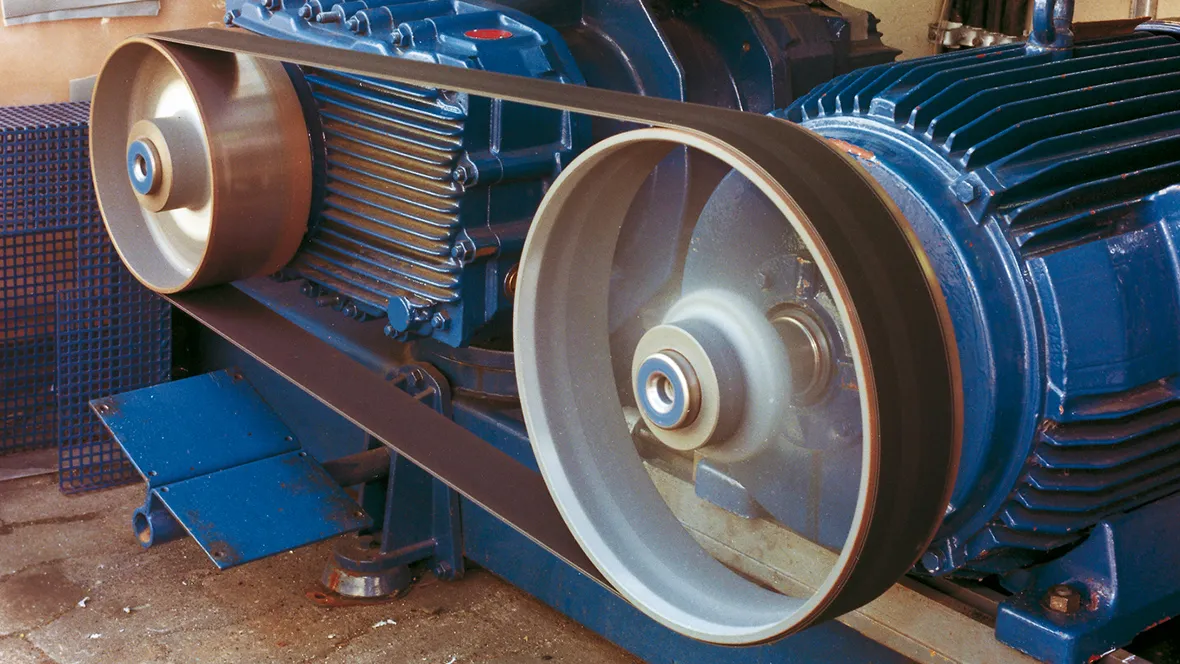
\includegraphics[width=.9\linewidth]{./pictures/flat-belt.png}
\end{center}
\end{frame}

\begin{frame}[label={sec:orgfa973e2}]{Types of Belts -- V Belts}
\begin{center}
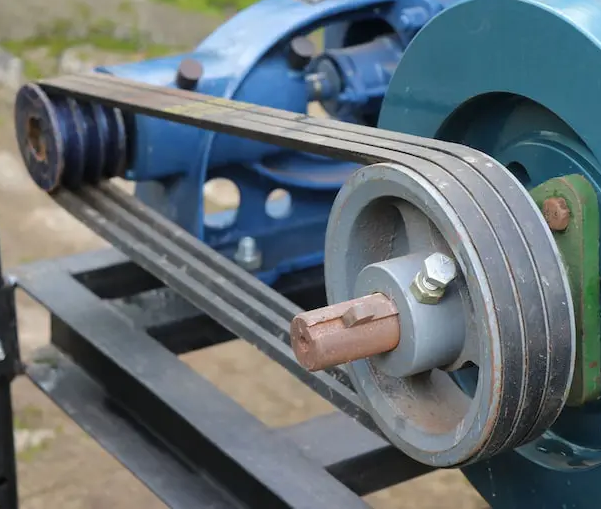
\includegraphics[width=.9\linewidth]{./pictures/v-belts.png}
\end{center}
\end{frame}

\begin{frame}[label={sec:org4c2ee01}]{Types of Belts -- Timing Belts}
\begin{center}
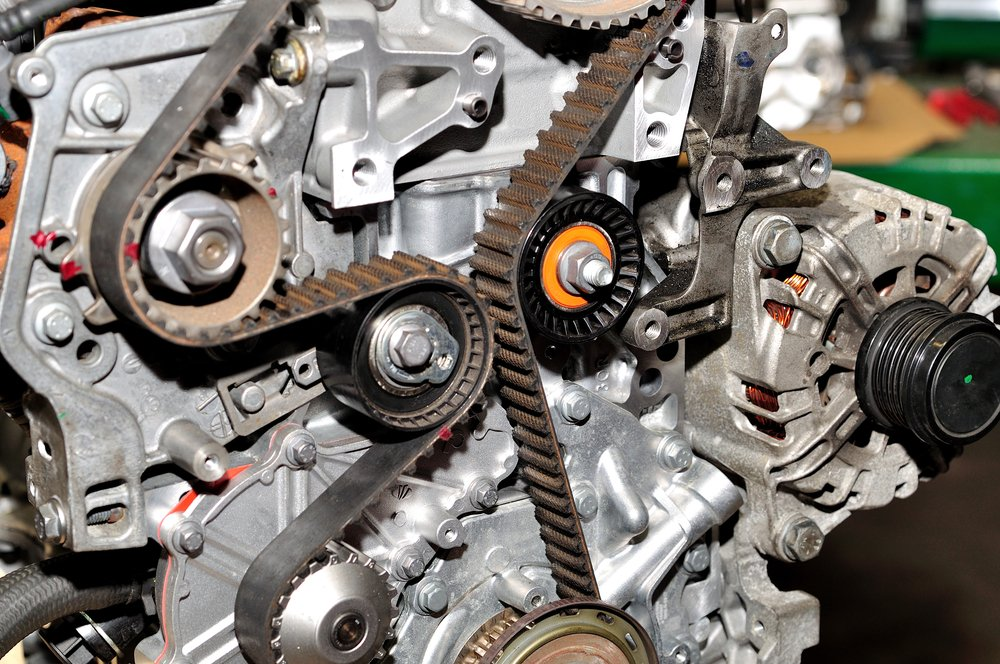
\includegraphics[width=.9\linewidth]{./pictures/timing-belt.jpg}
\end{center}
\end{frame}

\begin{frame}[label={sec:org16ace9f}]{Belt - Pulley Geometry}
\begin{center}
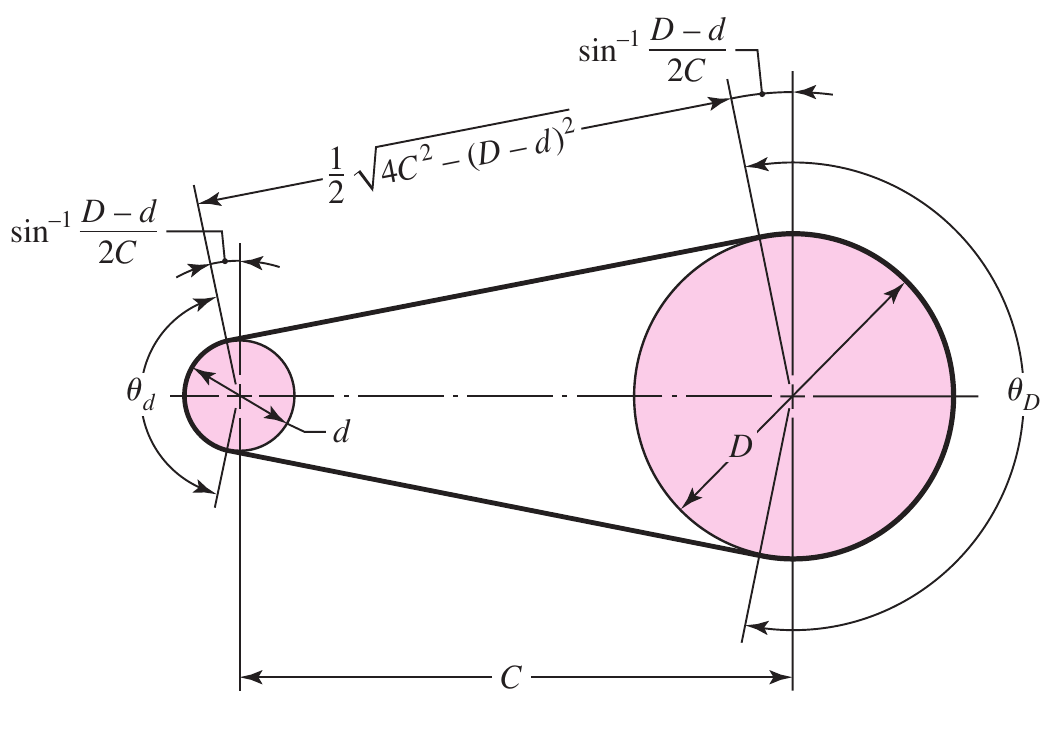
\includegraphics[width=0.7\textwidth]{./pictures/belt-pulley-geometry.png}
\end{center}
\vspace{-0.5cm}
\begin{align*}
    \theta_d &= \pi - 2 \sin^{-1} \frac{D - d}{2C} \\
    \theta_D &= \pi + 2 \sin^{-1} \frac{D - d}{2C} \\
    L &= \sqrt{ 4C^2 - (D - d)^2 } + \frac{1}{2}(D \theta_D + d \theta_d)
\end{align*}
\end{frame}

\begin{frame}[label={sec:org9e33eab}]{Cross Belt - Pulley Geometry}
\begin{center}
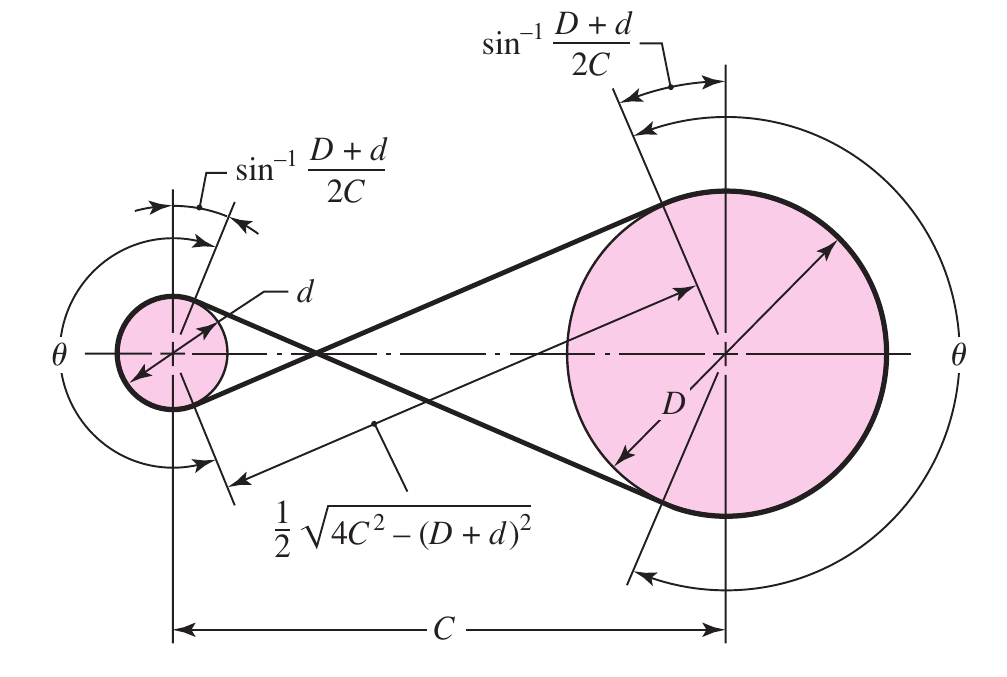
\includegraphics[width=0.7\textwidth]{./pictures/cross-belt-pulley-geometry.png}
\end{center}
\vspace{-0.5cm}
\begin{align*}
    \theta_d &= \pi + 2 \sin^{-1} \frac{D + d}{2C} \\
    L &= \sqrt{ 4C^2 - (D + d)^2 } + \frac{1}{2}(D + d)\theta
\end{align*}
\end{frame}

\section{Flat Belts}
\label{sec:org2545be6}

\begin{frame}[label={sec:orgc4d88e0}]{Flat Belts}
Uses: light-duty + long-distance power transmission

Strength:
\begin{itemize}
\item High performance (less friction involved)
\item Easy to install
\item Flat surface means less wear and energy loss from friction
\end{itemize}

Weakness:
\begin{itemize}
\item Need high belt tension
\item Shortened bearing life
\item Tendency to climb
\end{itemize}
\end{frame}

\begin{frame}[label={sec:orgb586fc7}]{Flat Belt Assembly}
\begin{itemize}
\item Typically paired with crowned pulleys
\item Keep belt centered
\end{itemize}

\begin{center}
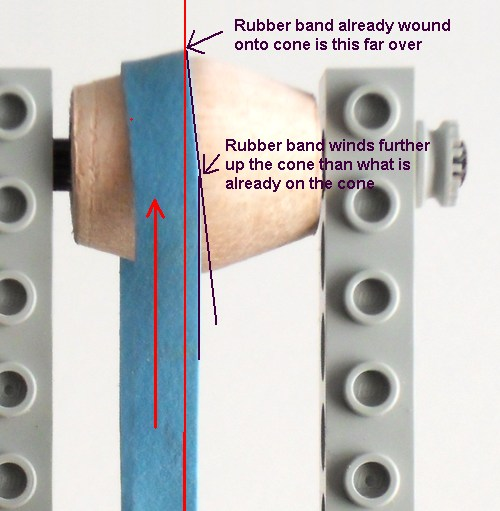
\includegraphics[height=0.8\textheight]{./pictures/crowned-pulley.jpg}
\end{center}
\end{frame}

\begin{frame}[label={sec:orga8718d1}]{Belt Tension}
\begin{itemize}
\item For high speed belt drive

\begin{align*}
    \frac{F_1 - F_c}{F_2 - F_c} = e^{\mu \theta}
\end{align*}

where \(F_c = m \omega^2 r^2\) is the centrifugal force on the belt
and \(m\) is the \alert{mass per length} of belt
\end{itemize}
\end{frame}

\begin{frame}[label={sec:org9575184}]{Force Balance on Pulley}
\begin{center}
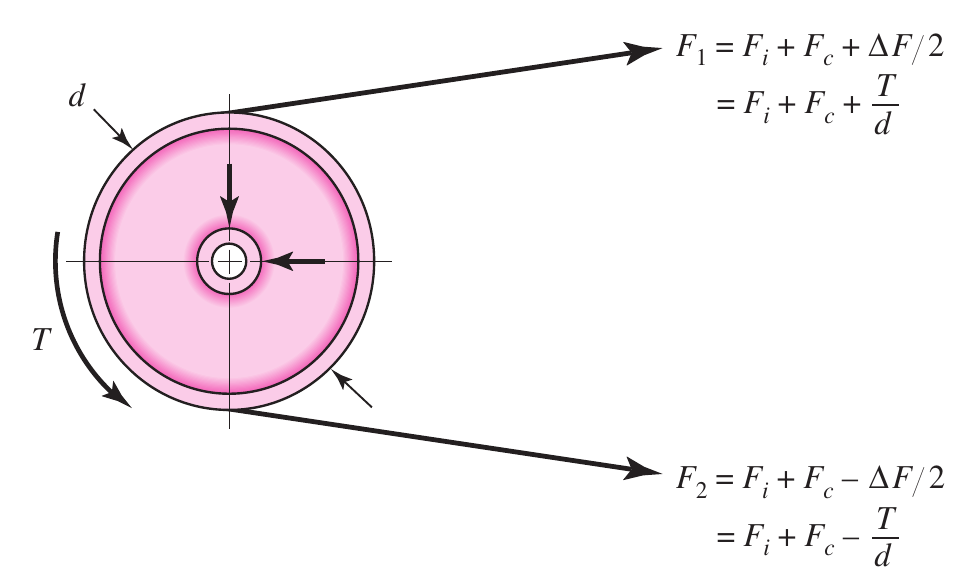
\includegraphics[height=0.5\textheight]{./pictures/forces-on-pulley.png}
\end{center}

\begin{align*}
  F_{1} - F_{2} &= \frac{2T}{d} \\
  F_{1} + F_{2} &= 2F_{i} + 2F_{c} \\
  F_{i} &= \frac{F_{1} + F_{2}}{2} + F_{c}
\end{align*}
\end{frame}

\begin{frame}[label={sec:org647f61a}]{Initial Belt Tension \(F_{i}\)}
\begin{align*}
  \frac{F_{i}}{T/d} &= \frac{(F_{1} + F_{2})/2 - F_{c}}{(F_{1} - F_{2})/2} = \frac{F_{1} + F_{2} - 2F_{c}}{F_{1} - F_{2}} \\
                    &= \frac{(F_{1} - F_{c}) + (F_{2} - F_{c})}{(F_{1} - F_{c}) - (F_{2} - F_{c})} \\
                    &= \frac{(F_{1} - F_{c})/(F_{2} - F_{c}) + 1}{(F_{1} - F_{c})/(F_{2} - F_{c}) - 1} \\
                    &= \frac{e^{\mu\theta} + 1}{e^{\mu\theta} - 1} \\
  F_{i} &= \frac{T}{d}\frac{e^{\mu \theta} + 1}{e^{\mu \theta} - 1}
\end{align*}

\begin{itemize}
\item Note: \(F_{i} = 0 \rightarrow T = 0\)
\end{itemize}
\end{frame}

\begin{frame}[label={sec:org85ffcf2}]{Tight and Slack Side Tensions}
\begin{align*}
  F_{1} &= F_{c} + F_{i} + \frac{T}{d} = F_{c} + F_{i} + F_{i} \frac{e^{\mu\theta} - 1}{e^{\mu\theta} + 1} \\
        &= F_{c} + F_{i}\frac{\left( e^{\mu\theta} + 1 + e^{\mu\theta} - 1 \right)}{e^{\mu\theta} + 1} \\
        &= F_{c} + F_{i}\frac{2e^{\mu\theta}}{e^{\mu\theta} + 1} \\
  F_{2} &= F_{c} + F_{i}\frac{2}{e^{\mu\theta} + 1} \\
\end{align*}

\begin{itemize}
\item Power transmitted

$$H = (F_1 - F_2) v$$
\end{itemize}
\end{frame}

\begin{frame}[label={sec:org061c7db}]{Belt Design}
\begin{align*}
    (F_1)_a &= b F_a C_p C_v \\
\end{align*}
\begin{align*}
    \left( F_1 \right)_a &= \text{allowable largest tension} \\
    b &= \text{belt width} \\
    F_a &= \text{manufacturer's allowed tension per width (N/m)} \\
    C_p &= \text{pulley correction factor} \\
    C_v &= \text{velocity correction factor = 1 except leather belts}
\end{align*}
\end{frame}

\begin{frame}[label={sec:org9c89844}]{Manufacturer's Allowed Tension: \(F_a\)}
\begin{center}
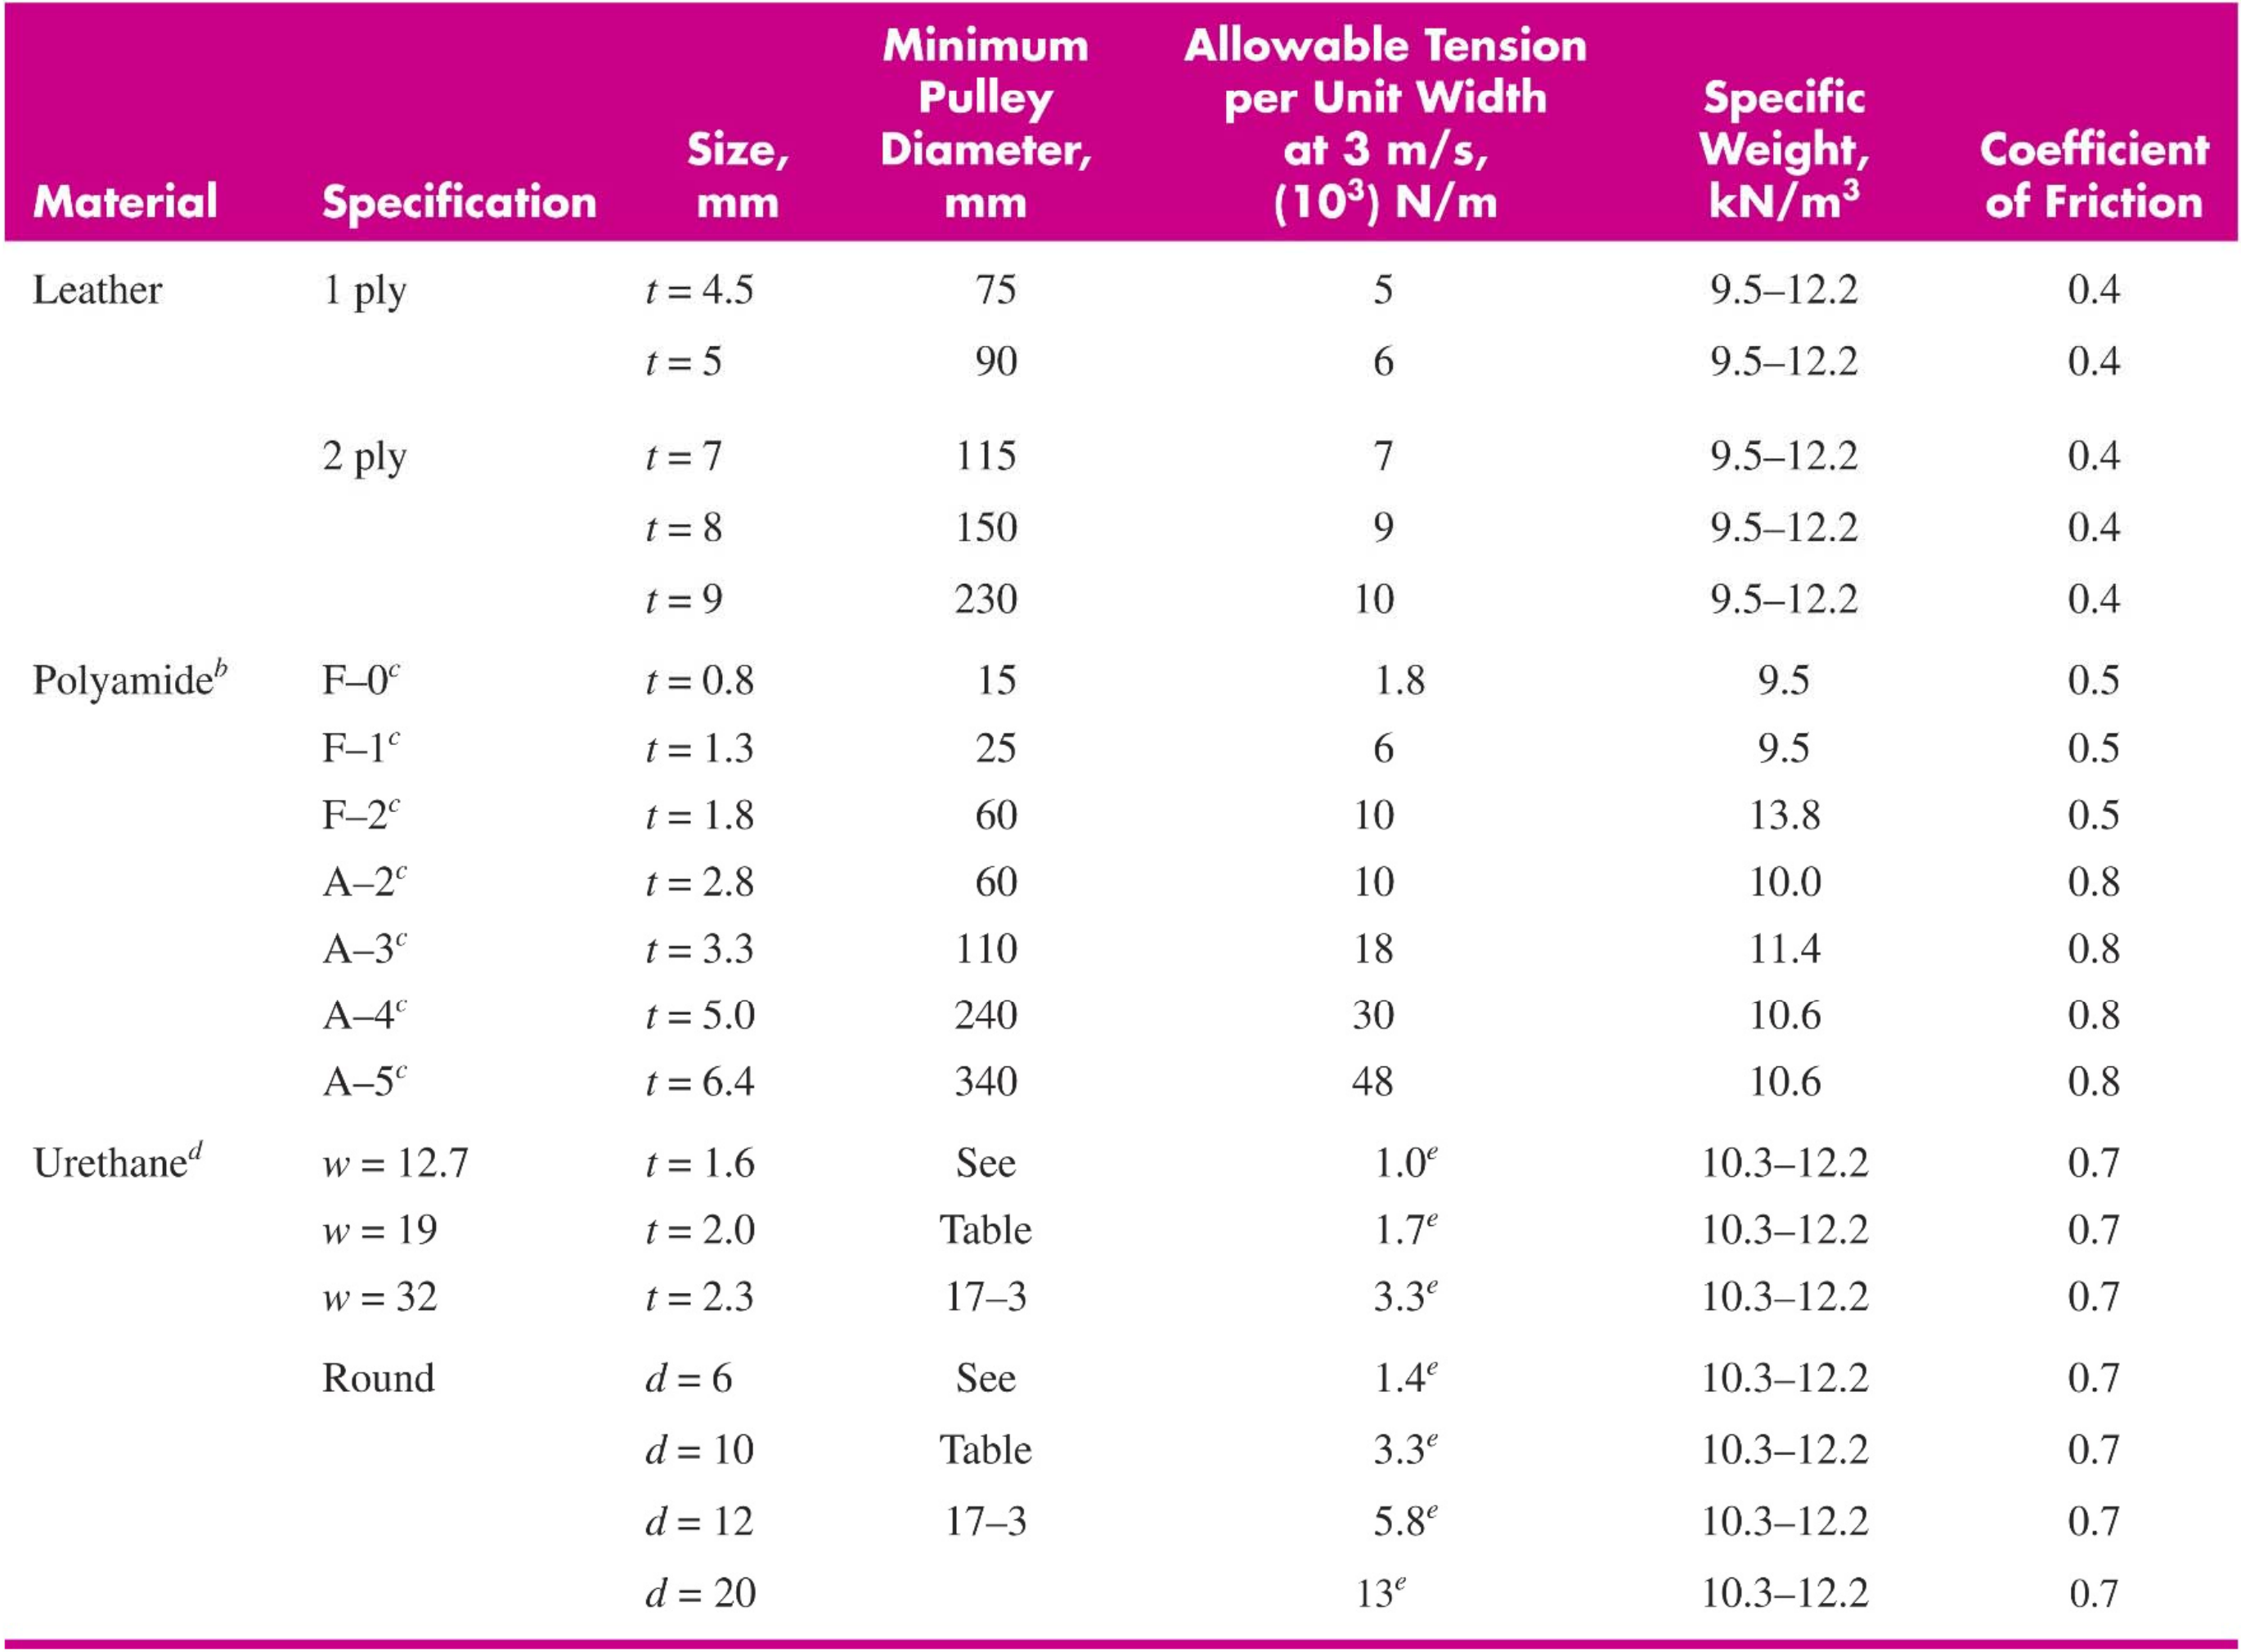
\includegraphics[width=\textwidth]{./pictures/belt-allowable-tension.png}
\end{center}
\end{frame}

\begin{frame}[label={sec:orgd6ce725}]{Pulley Correction Factor: \(C_p\)}
\begin{center}
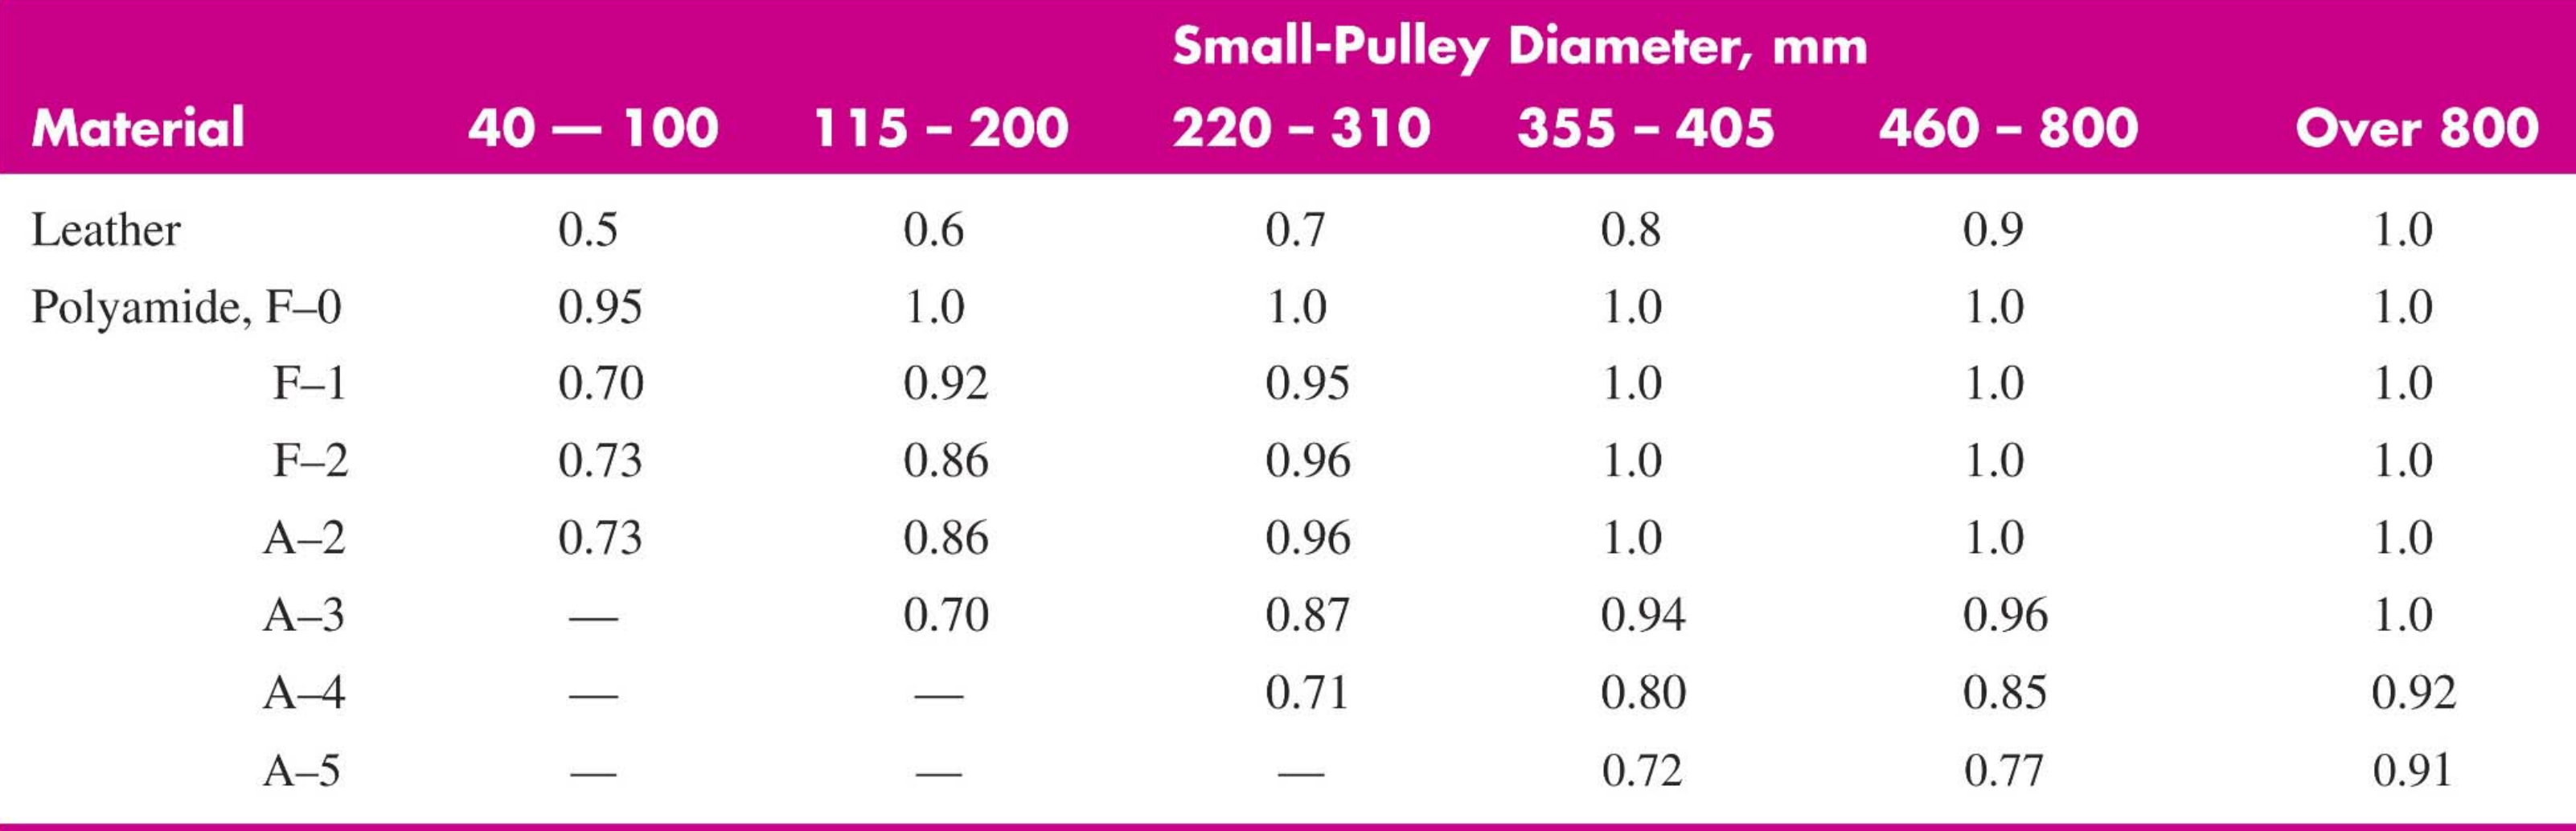
\includegraphics[width=\textwidth]{./pictures/pulley-correction-factor.png}
\end{center}

\begin{itemize}
\item \(C_p\) = 1 for urethane belts
\end{itemize}
\end{frame}

\begin{frame}[label={sec:orgdcf1b81}]{Velocity Correction Factor: \(C_v\)}
\begin{center}
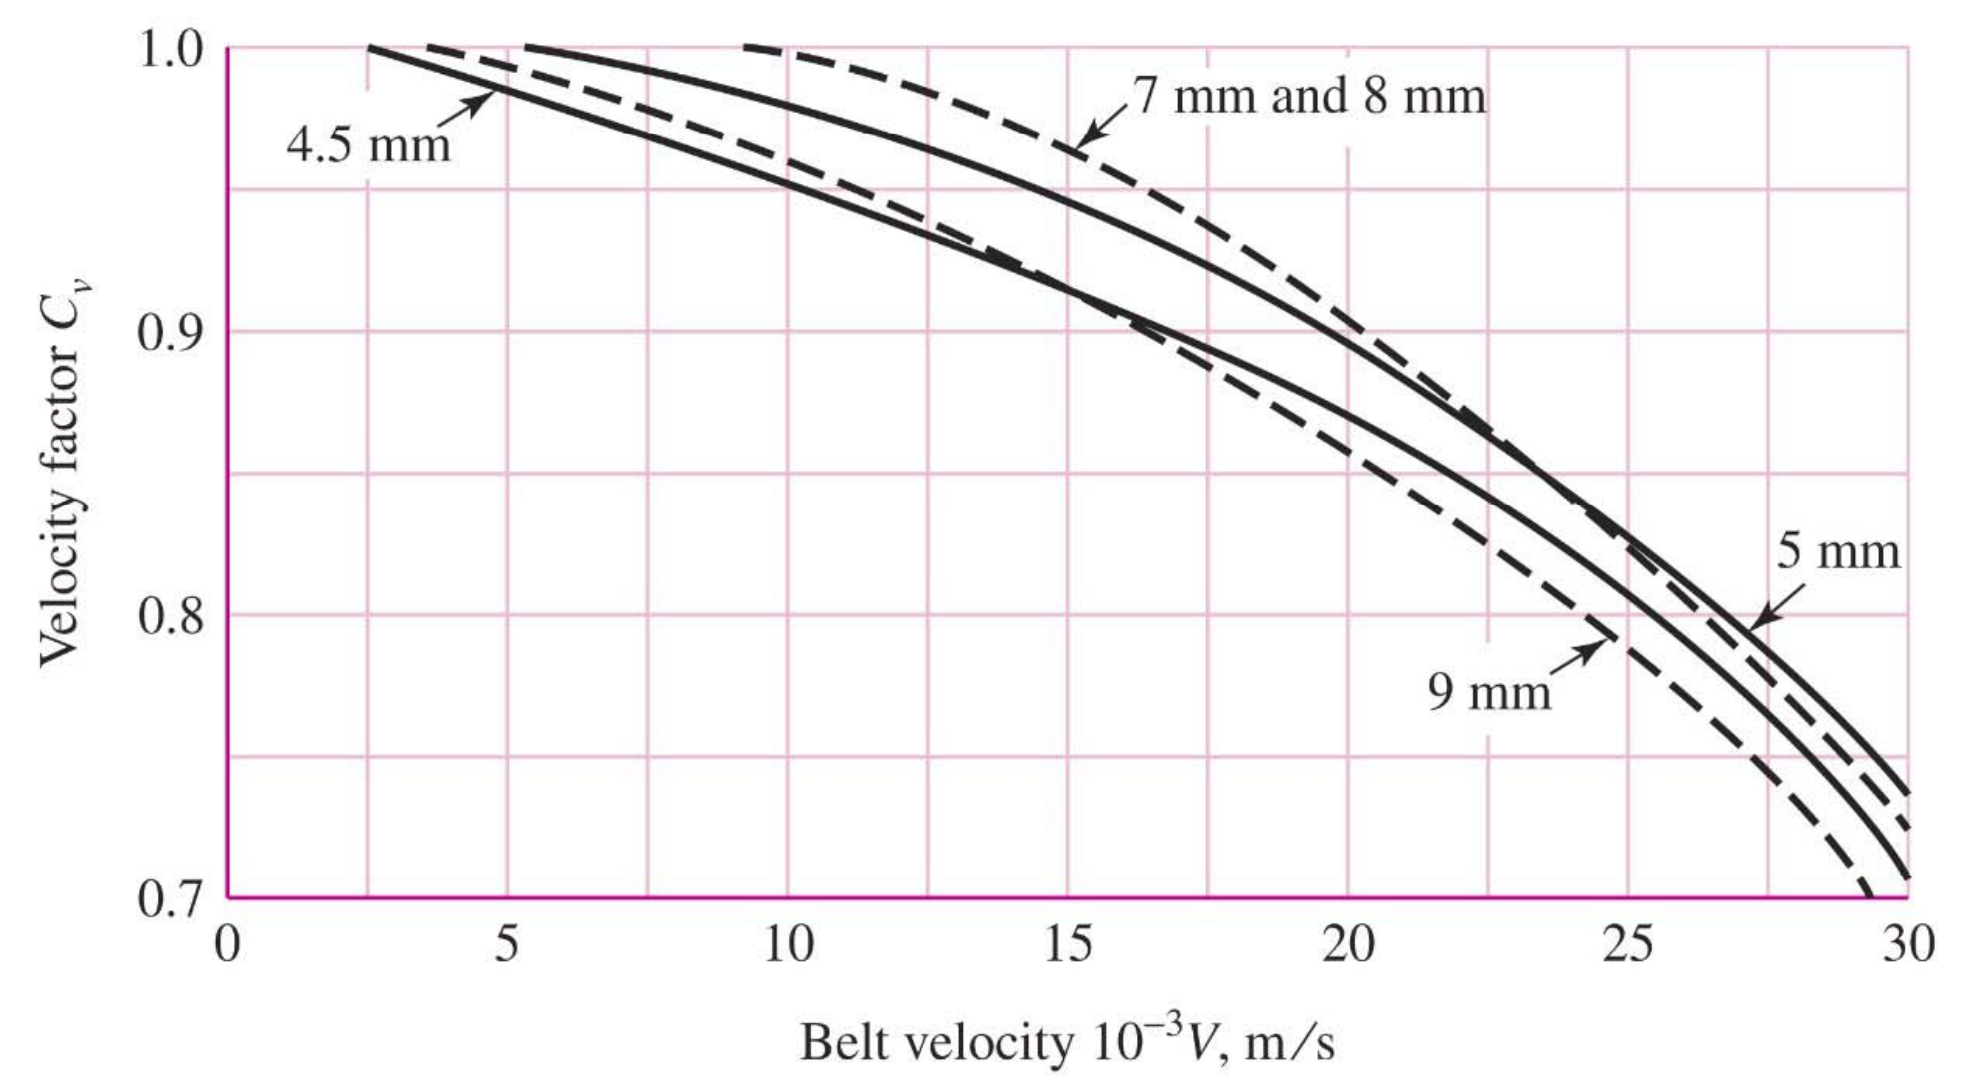
\includegraphics[width=\textwidth]{./pictures/velocity-correction-factor.png}
\end{center}

\begin{itemize}
\item \(C_v\) = 1 for polyamide and urethane belts
\end{itemize}
\end{frame}

\begin{frame}[label={sec:org52e7e8d}]{Example: Flat belt design}
A polyamide A-3 flat belt 15 cm wide is used to transmit 15 hp power. The pulley rotational axes are parallel, the shafts are 2.5 m apart. The driving pulley diameter is 15 cm and rotates at 1750 rpm. The driven pulley diameter is 45 cm.

\begin{enumerate}
\item Estimate the centrifugal tension \(F_c\)
\item Determine the required initial tension \(F_{i}\)
\item Estimate the allowable \(F_1\) and \(F_2\)
\end{enumerate}
\end{frame}

\begin{frame}[label={sec:org03fa7b0}]{Solution: Flat belt design (1)}
Find \(F_c\)

\begin{align*}
\gamma &= 11.4 \text{ kN/m}^3 \\
\rho &= \frac{\gamma}{g} = 11.4 \times 10^3 / 9.81 = 1.162 \times 10^3 \text{ kg/m}^3 \\
m &= \rho A = 1.162 \times 10^3 (3.3 \times 10^{-3})(0.15) = 0.575 \text{ kg/m} \\
F_c &= m \omega^2 r^2 = 0.575 \times (1750 (2\pi/60))^2 (0.15/2)^2 = 108.6 \text{ N}
\end{align*}
\end{frame}

\begin{frame}[label={sec:org6b379a6}]{Solution: Flat belt design (2)}
First, find \(\theta\) on the smaller pulley (smaller pulley = smaller angle)
\begin{align*}
    \theta_{d} &= \pi - 2\sin^{-1}\frac{D-d}{2C} \\
               &= \pi - 2\sin^{-1}\frac{45 - 15}{2(250)} \\
               &= 3.02 \text{ rad}
\end{align*}

Next, find input torque \(T\)
\begin{align*}
    T &= \frac{H}{\omega} = \frac{15(746)}{1750\frac{2\pi}{60}} \\
      &= 61.1 \text{ N-m}
\end{align*}
\end{frame}

\begin{frame}[label={sec:orga06803b}]{Solution: Flat belt design (2)}
Finally,
\begin{align*}
    F_{i} &= \frac{T}{d}\frac{e^{\mu\theta} + 1}{e^{\mu\theta} - 1} \\
          &= \frac{61.1}{0.15}\frac{e^{0.8(3.02)} + 1}{e^{0.8(3.02)} - 1} \\
          &= 487 \text{ N}
\end{align*}
\end{frame}

\begin{frame}[label={sec:org9509d9a}]{Solution: Flat belt design (3)}
For \(F_1\) and \(F_2\)

\begin{align*}
    F_{1} &= F_{c} + F_{i} \frac{2e^{\mu\theta}}{e^{\mu\theta}+1} \\
         &= 108.6 + 487\frac{2e^{0.8(3.02)}}{e^{0.8(3.02)}+ 1} \\
         &= 1003 \text{ N} \\
    F_{2} &= F_{c} + F_{i} \frac{2}{e^{\mu\theta}+1} \\
         &= 108.6 + 487\frac{2}{e^{0.8(3.02)}+ 1} \\
         &= 188.4 \text{ N}
\end{align*}
\end{frame}
\section{V-Belts}
\label{sec:orgb0d2d03}

\begin{frame}[label={sec:org80dccf5}]{Why V Belts?}
\begin{itemize}
\item Increased tension forces belt further into groove, providing more friction
\item More friction \(\rightarrow\) increased torque capacity, but at lower efficiency and increased rate of wear
\end{itemize}
\end{frame}

\begin{frame}[label={sec:org32fc6f1}]{V Belt Application}
\begin{center}
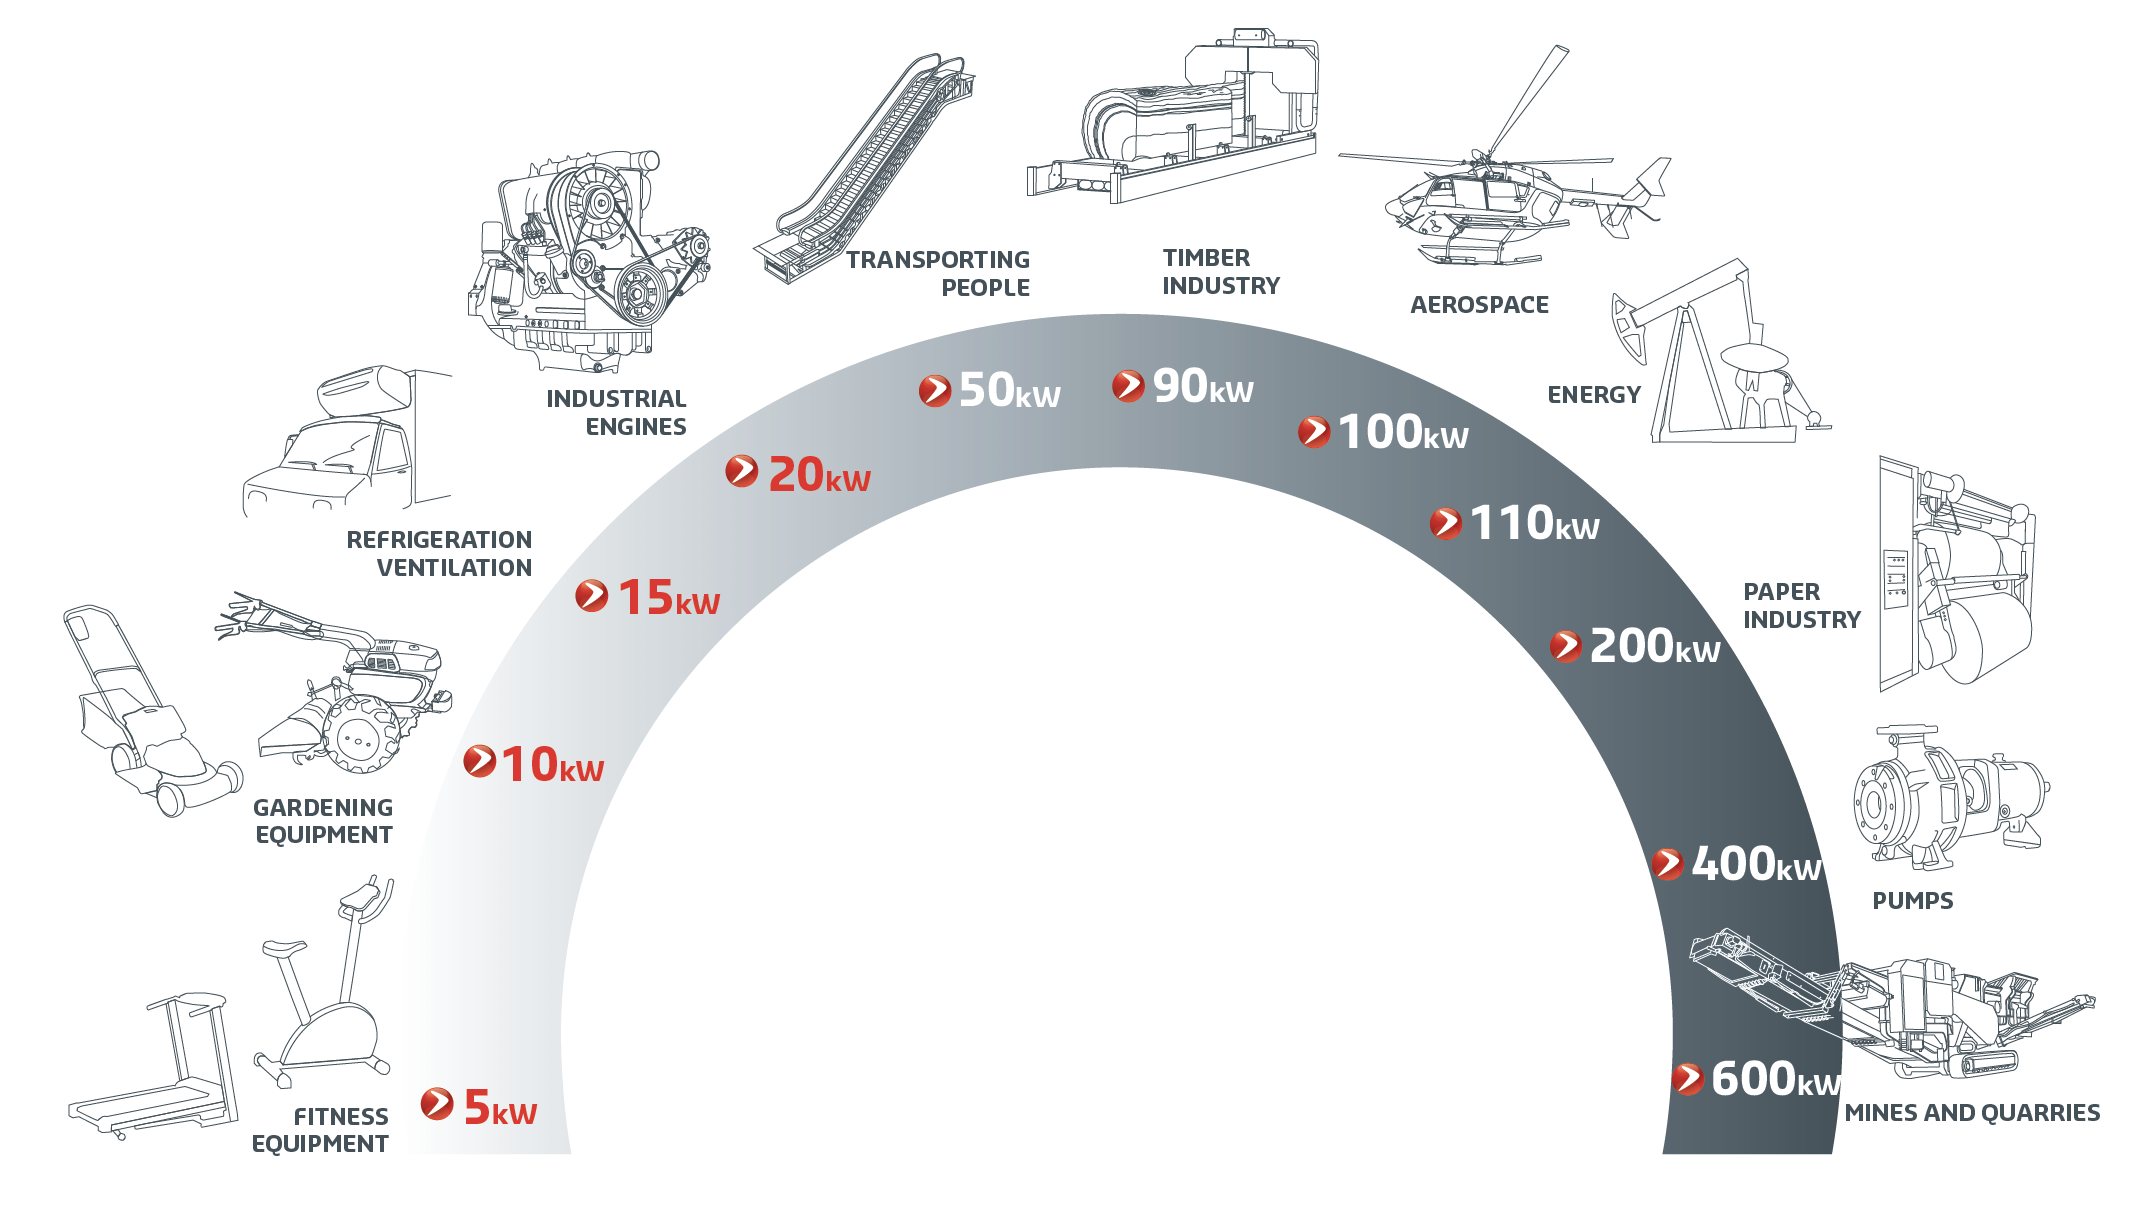
\includegraphics[width=\textwidth]{./pictures/v-belt-applications.png}
\end{center}
\end{frame}

\begin{frame}[label={sec:org060cc28}]{V Belt Sections}
\begin{center}
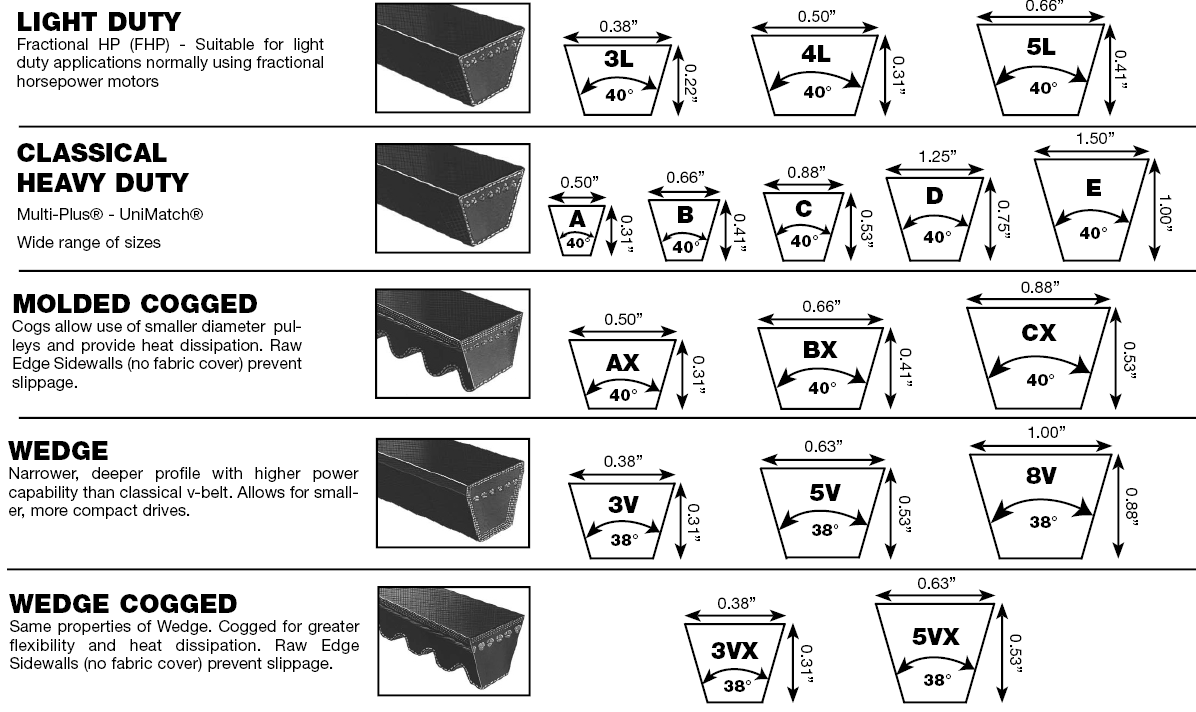
\includegraphics[width=.9\linewidth]{./pictures/v-belt-sections.png}
\end{center}
\end{frame}

\begin{frame}[label={sec:orgcf7433d}]{V Belt Tension}
\begin{itemize}
\item Similar equations to flat belts
\item Minor adjustment for groove angle \(\beta \approx 40^{\circ}\)

\begin{gather*}
    T = \left( F_1 - F_2 \right) r \\
    H = \left( F_1 - F_2 \right) v \\
    \frac{F_1 - F_c}{F_2 - F_c} = e^{\dfrac{\mu \theta}{\sin (\beta/2)}}
\end{gather*}
\end{itemize}
\end{frame}

\begin{frame}[label={sec:org528adc9}]{V Belt Design Equation}
\begin{itemize}
\item Determine based on belt speed and power requirement
\end{itemize}

\begin{align*}
  N_s = \frac{H_a n}{H K_s}
\end{align*}

\begin{description}
\item[{\(N_s\)}] safety factor
\item[{\(H_a\)}] allowable power per belt
\item[{\(n\)}] number of belts
\item[{\(H\)}] actual power = \((F_1 - F_2)v\)
\item[{\(K_s\)}] service factor
\end{description}
\end{frame}

\begin{frame}[label={sec:org87f8442}]{Allowable Power (\(H_a\)) in KW per belt}
\vspace{-2mm}
\begin{center}
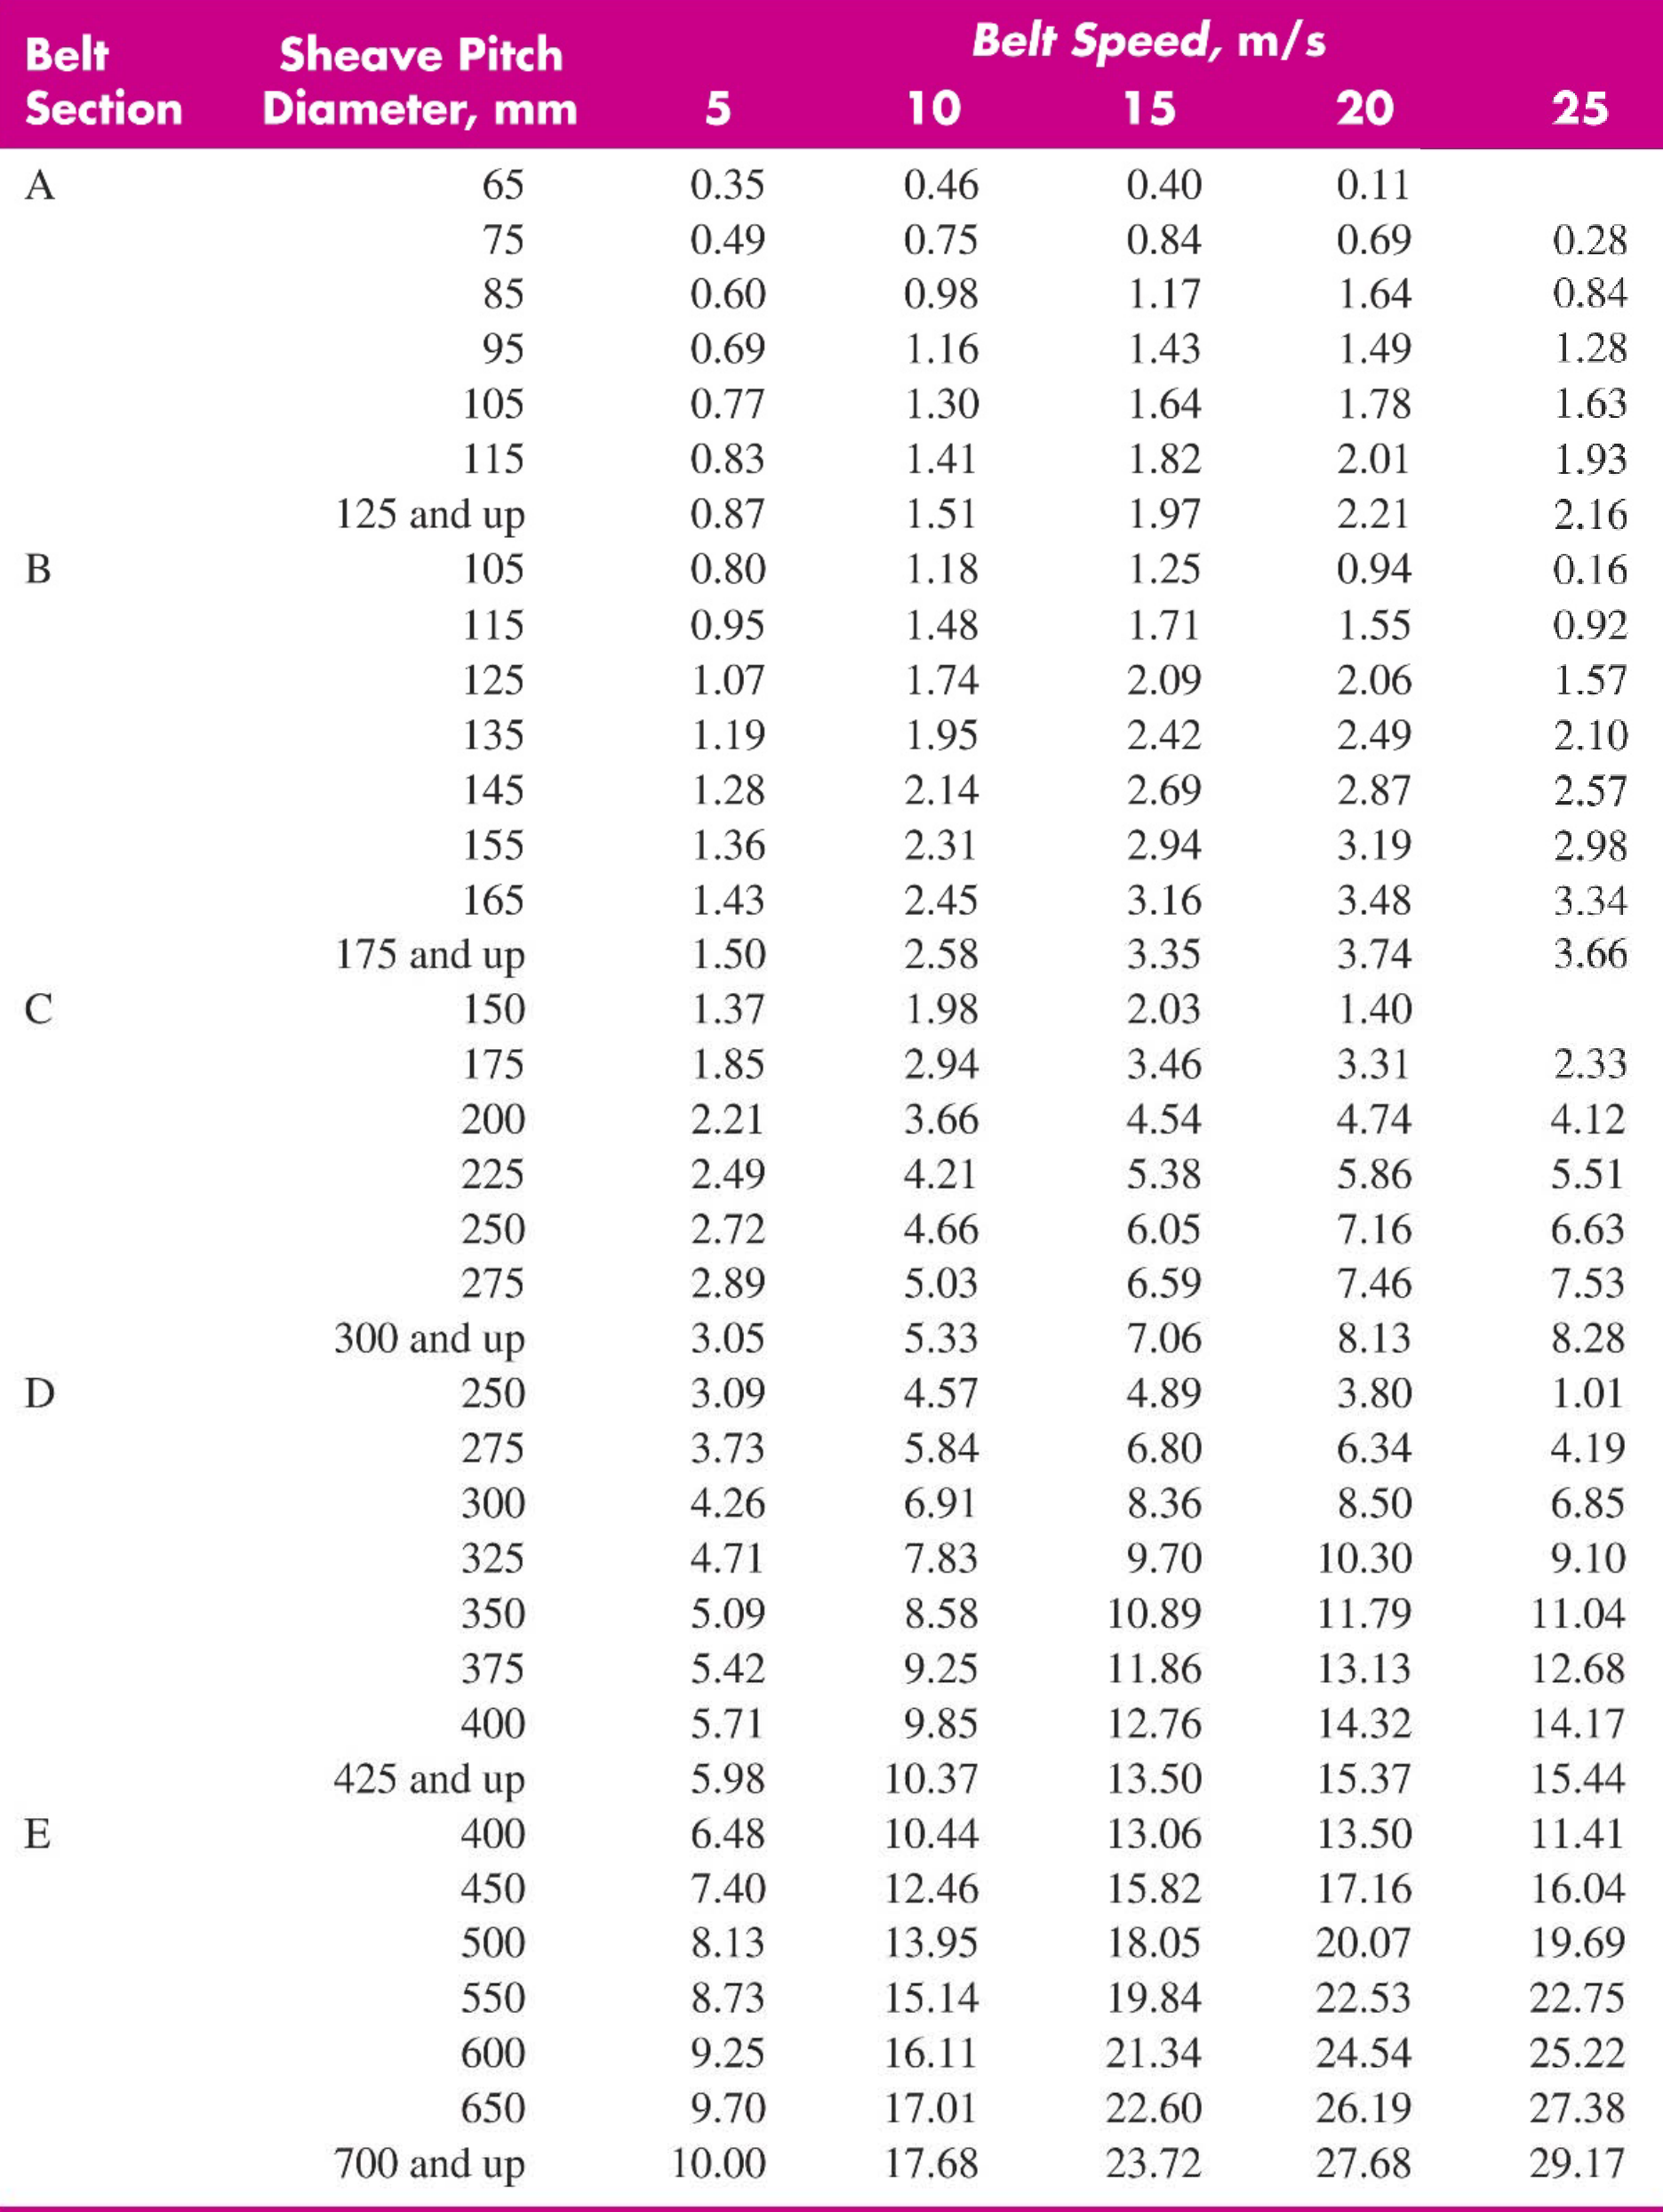
\includegraphics[width=0.6\textwidth]{./pictures/belt-power-rating.png}
\end{center}
\end{frame}

\begin{frame}[label={sec:org40db861}]{Service Factor}
\begin{center}
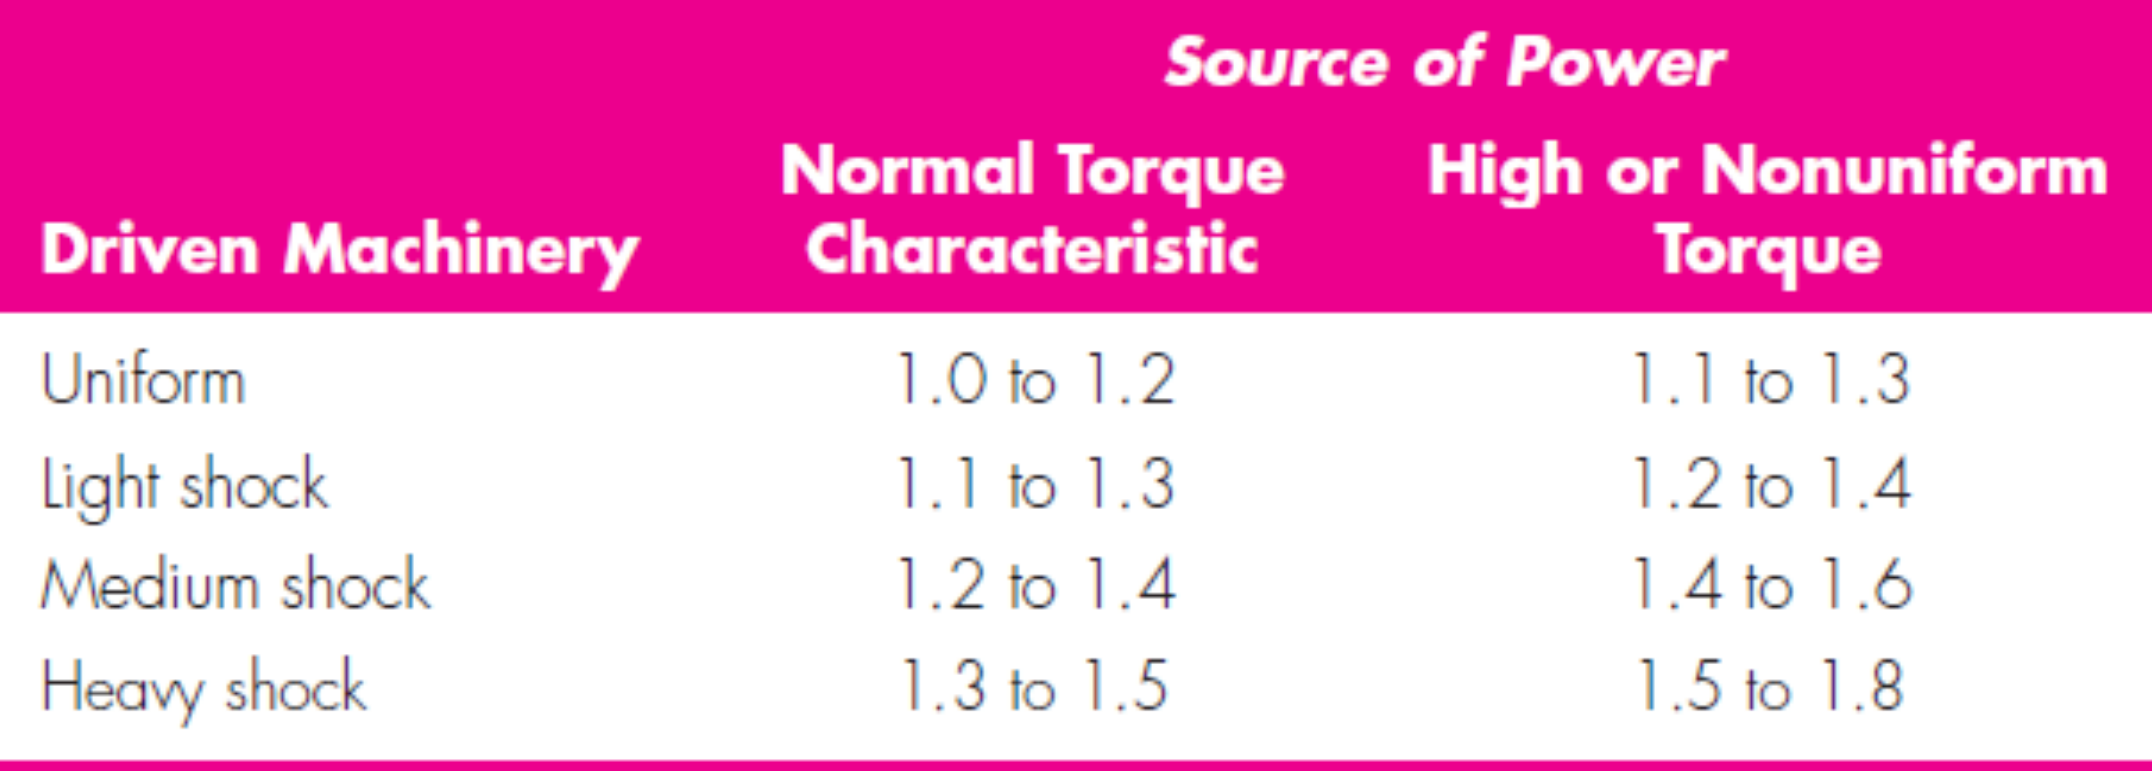
\includegraphics[width=0.7\textwidth]{./pictures/belt-service-factor.png}
\end{center}
\end{frame}

\begin{frame}[label={sec:orgfb20dec}]{Example: V Belt Design}
A 5-hp gasoline engine is connected to a water pump by v-belt and sheaves at 2000 rpm. The driving sheave has \(d\) = 200 mm. Choose a proper belt section and the number of belts for the job with \(N_s\) = 1.5.
\end{frame}

\begin{frame}[label={sec:org2871c17}]{Solution: V Belt Design}
\begin{itemize}
\item Belt speed \(v\) is
\begin{align*}
  v &= 2000 \left(\frac{2\pi}{60}\right) (0.2/2) \\
    &= 20.94 \text{ m/s}
\end{align*}

\item Gasoline engines are usually classified as 'medium' shock

\begin{align*}
  H_{a} &= N_{s} \frac{HK_{s}}{n} \\
        &= 1.5 \frac{5(746)(1.4)}{1} \\
        &= 7833 \text{ W} = 7.83 \text{ kW}
\end{align*}
\end{itemize}
\end{frame}

\begin{frame}[label={sec:org1fa3ccb}]{Solution: V Belt Design}
\begin{itemize}
\item As \(d\) =  200 mm, we are limited to sections A, B, and C

\item v = 20.94 m/s (round down to 20 m/s) \(\rightarrow\) 4th column

\item for section C, \(d\) = 200, \(H_a\) = 4.74 kW \(\rightarrow\) 2 belts
\item for section B, \(d\) = 200, \(H_a\) = 3.74 kW \(\rightarrow\) 3 belts
\item for section A, \(d\) = 200, \(H_a\) = 2.21 kW \(\rightarrow\) 4 belts
\end{itemize}
\end{frame}

\begin{frame}[label={sec:orgc3b8180}]{Timing Belts}
\begin{center}
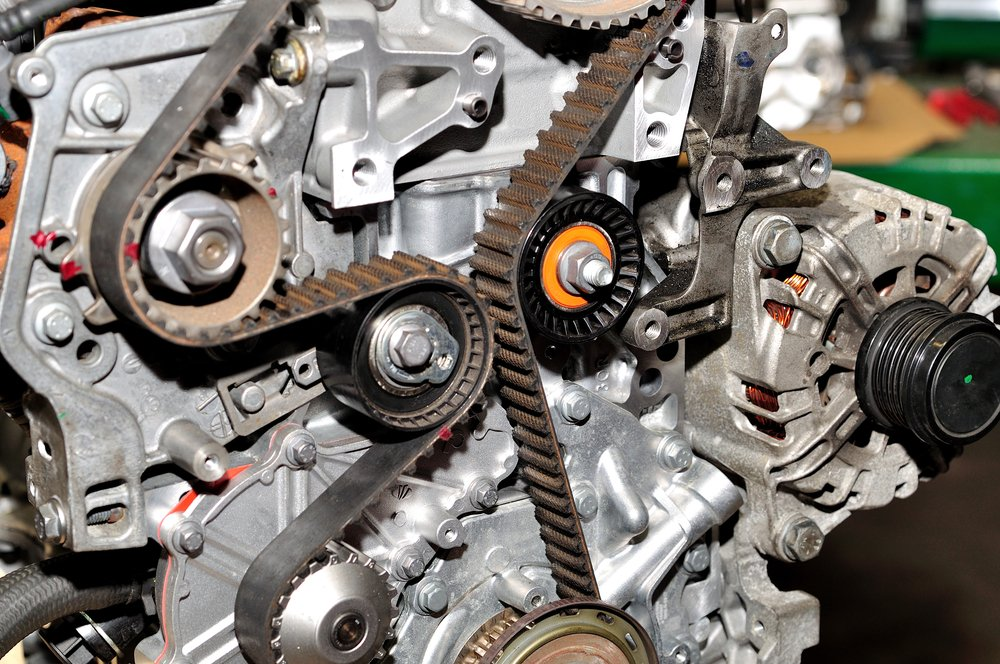
\includegraphics[width=.9\linewidth]{./pictures/timing-belt.jpg}
\end{center}
\begin{itemize}
\item No significant stretch or slip \(\rightarrow\) power where speed ratio is important
\item efficiency of 97 - 99\%
\item No need for lubrication
\item Quieter than chain drives
\item Same design equations as V-belts
\end{itemize}
\end{frame}

\section{Roller Chains}
\label{sec:org90331cd}

\begin{frame}[label={sec:org0c6e00a}]{Roller Chain Components}
\begin{center}
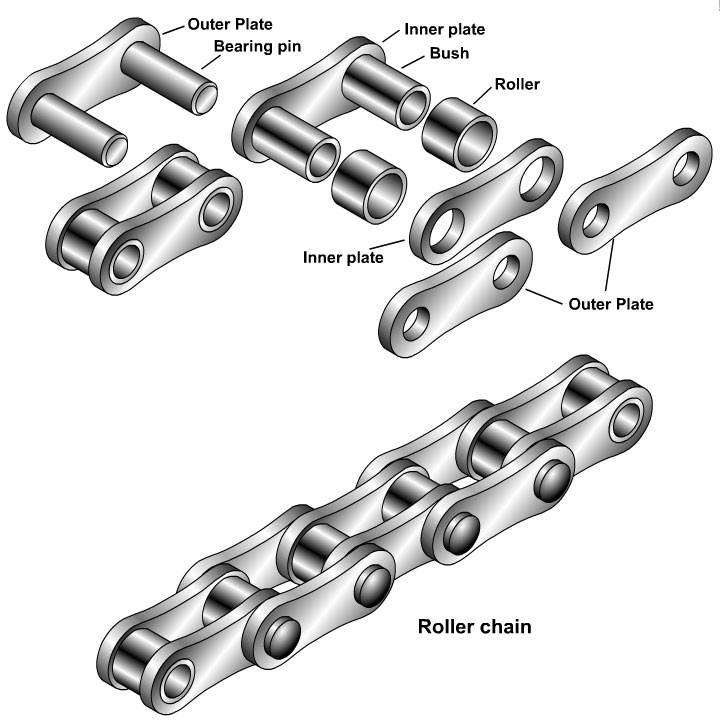
\includegraphics[height=0.9\textheight]{./pictures/roller-chain-parts.jpg}
\end{center}
\end{frame}

\begin{frame}[label={sec:org7ae407c}]{Why Roller Chain (Chain Drives)?}
\begin{itemize}
\item No slip \(\rightarrow\) constant ratio
\item Long life
\item Can drive multiple shafts from a single source
\end{itemize}
\end{frame}

\begin{frame}[label={sec:org29f57c5}]{Forces and Powers}
\begin{itemize}
\item Chain tension only on tight side

$$ T = \frac{F_{1}D}{2} $$
$$ H = Fv $$
\end{itemize}
\end{frame}

\begin{frame}[label={sec:org528d247}]{Equations on Roller Chains}
\begin{columns}
\begin{column}{0.5\columnwidth}
\begin{center}
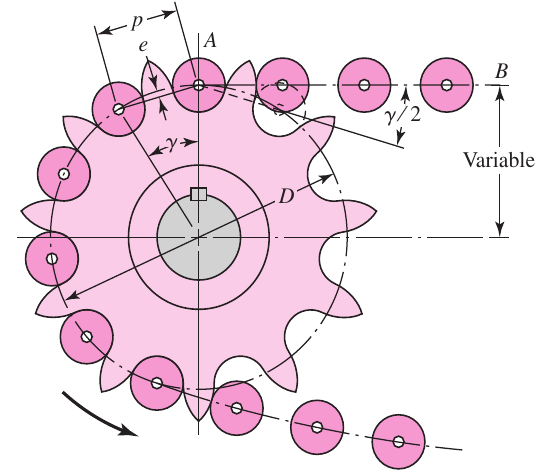
\includegraphics[height=\textwidth]{./pictures/chordal-speed-variation.png}
\end{center}
\end{column}

\begin{column}{0.5\columnwidth}
$$ D = \frac{p}{\sin \left( \dfrac{180^{\circ}}{N} \right)} = \frac{p}{\sin \left(\dfrac{\gamma}{2} \right)} $$
$$ v = N pn $$

\begin{description}
\item[{\(v\)}] velocity
\item[{\(N\)}] number of sprocket teeth
\item[{\(p\)}] chain pitch
\item[{\(n\)}] sprocket speed [rev/min]
\end{description}
\end{column}
\end{columns}
\end{frame}

\begin{frame}[label={sec:org65bf7b7}]{Chordal Speed Variation}
\begin{columns}
\begin{column}{0.5\columnwidth}
\begin{center}
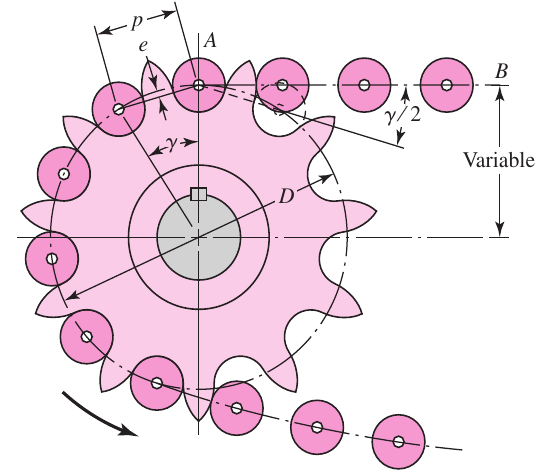
\includegraphics[height=\textwidth]{./pictures/chordal-speed-variation.png}
\end{center}
\end{column}

\begin{column}{0.5\columnwidth}
\begin{itemize}
\item max chain exit velocity

$$ v_{\max} = \pi D n = \frac{\pi n p}{\sin (\gamma/2)} $$

\item min chain exit velocity

$$ v_{\min} = \pi d n = \pi n p \frac{\cos(\gamma/2)}{\sin (\gamma/2)}$$

\item decrease \(\gamma\) to reduce variation
\end{itemize}
\end{column}
\end{columns}
\end{frame}

\begin{frame}[label={sec:orgd3362c8}]{Failure Mode}
\begin{itemize}
\item Because of speed variation and roller components, chains can fail from fatigue and wear
\end{itemize}

\begin{columns}
\begin{column}{0.5\columnwidth}
\begin{center}
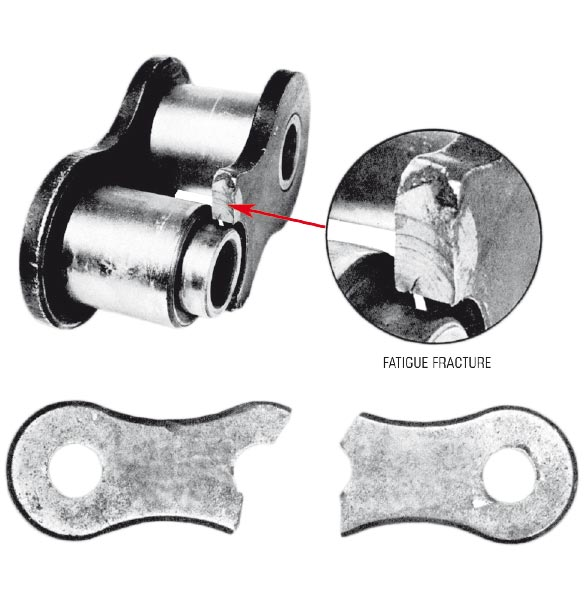
\includegraphics[width=.9\linewidth]{./pictures/link-plate-failure.jpg}
\end{center}

Link-plate failure from fatigue
\end{column}

\begin{column}{0.5\columnwidth}
\begin{center}
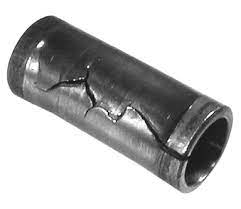
\includegraphics[width=.9\linewidth]{./pictures/roller-wear.jpg}
\end{center}

Roller wear/fatigue
\end{column}
\end{columns}
\end{frame}

\begin{frame}[label={sec:org18b1e66}]{Design Criteria}
\begin{itemize}
\item Roller chains rarely fail because of tensile stress
\item Need to worry more about fatigue and wear on rollers
\item To minimize chordal speed variation. \(N \geqslant 17\)
\end{itemize}
\end{frame}

\begin{frame}[label={sec:org151669d}]{Standard Chain Dimensions}
\begin{center}
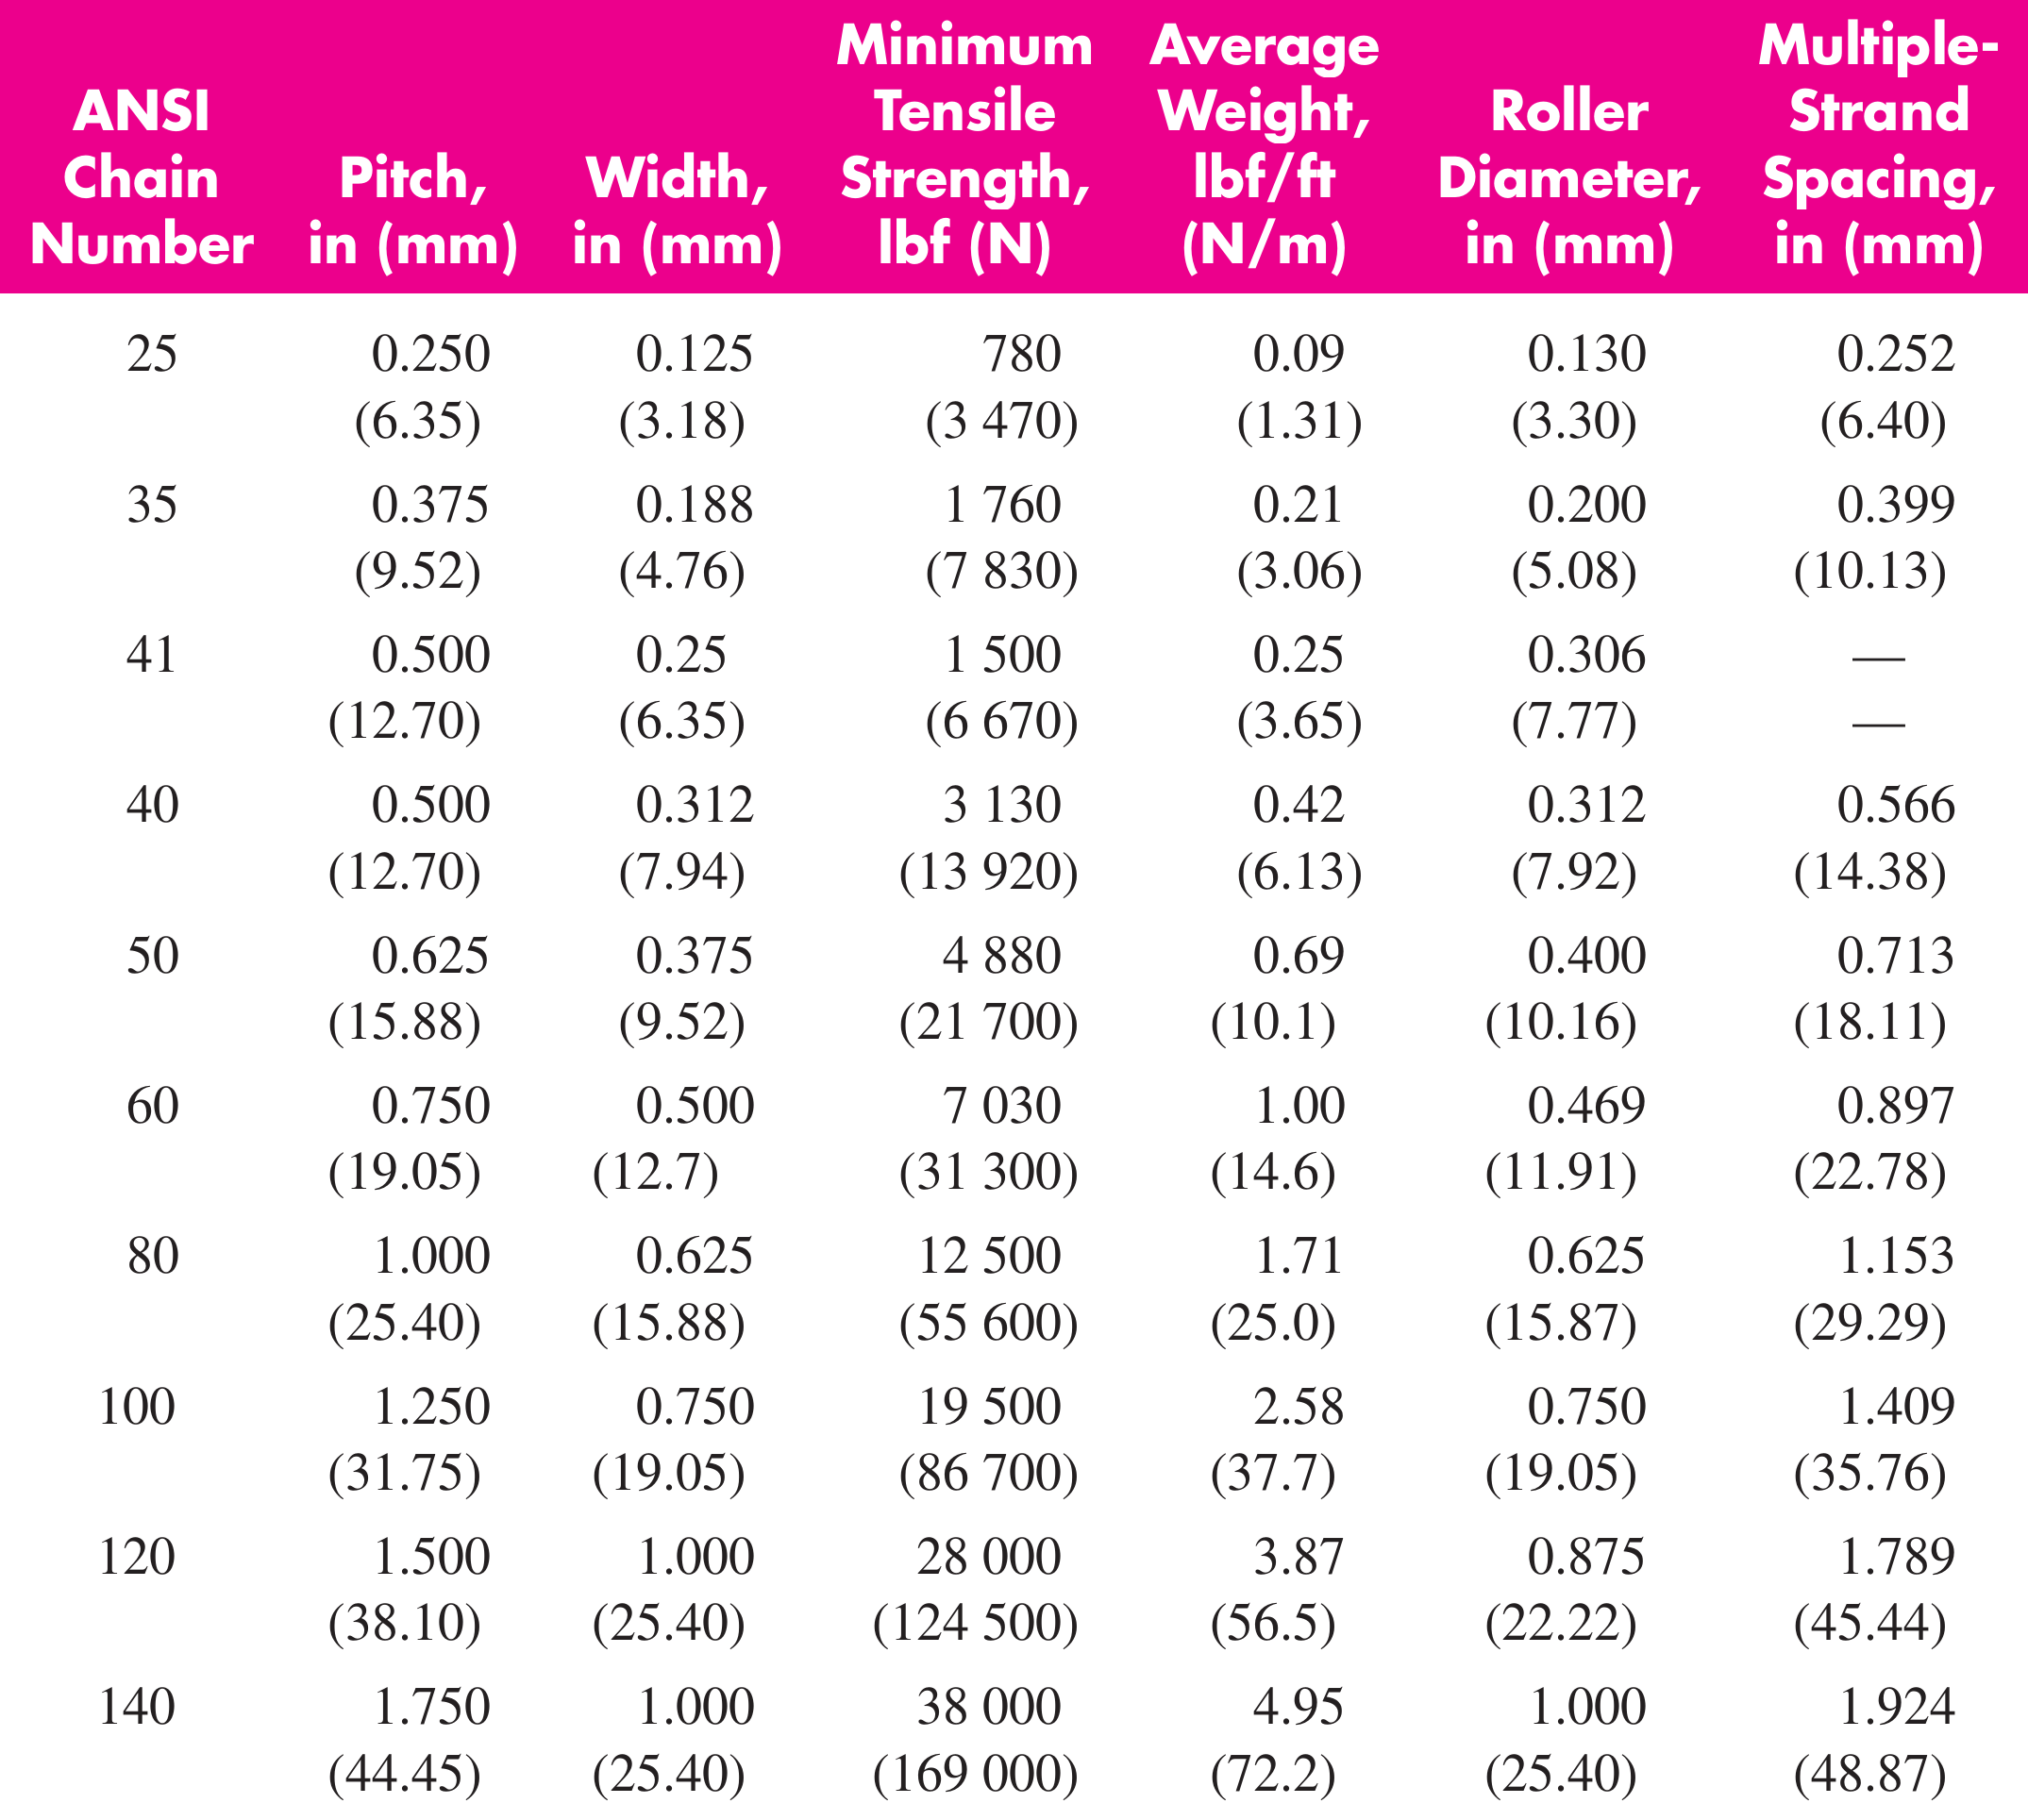
\includegraphics[height=0.9\textheight]{./pictures/chain-ansi-dims.png}
\end{center}
\end{frame}

\begin{frame}[label={sec:org4d8bb80}]{Power Capacity \(H\)}
\begin{itemize}
\item For link-plate limit
\end{itemize}

$$ H_1 = 0.004 N_1^{1.08} n_1^{0.9} p^{3-0.07p} \text{ hp} $$

\begin{itemize}
\item For roller limit
\end{itemize}

$$ H_2 = \frac{1000 K_t N_1^{1.5} p^{0.8}}{n_1^{1.5}} \text{ hp}$$

\begin{itemize}
\item \(N_1\) = number of teeth in smaller sprocket
\item \(n_1\) = sprocket speed [rev/min]
\item \(p\) = pitch of chain [m]
\item \(K_t\) = 29 for chain numbers 25,35; 3.4 for 41; and 17 for 40-240
\end{itemize}
\end{frame}

\begin{frame}[label={sec:org8ba60ac}]{Roller Chain Rated Capacity in hp (1)}
\begin{center}
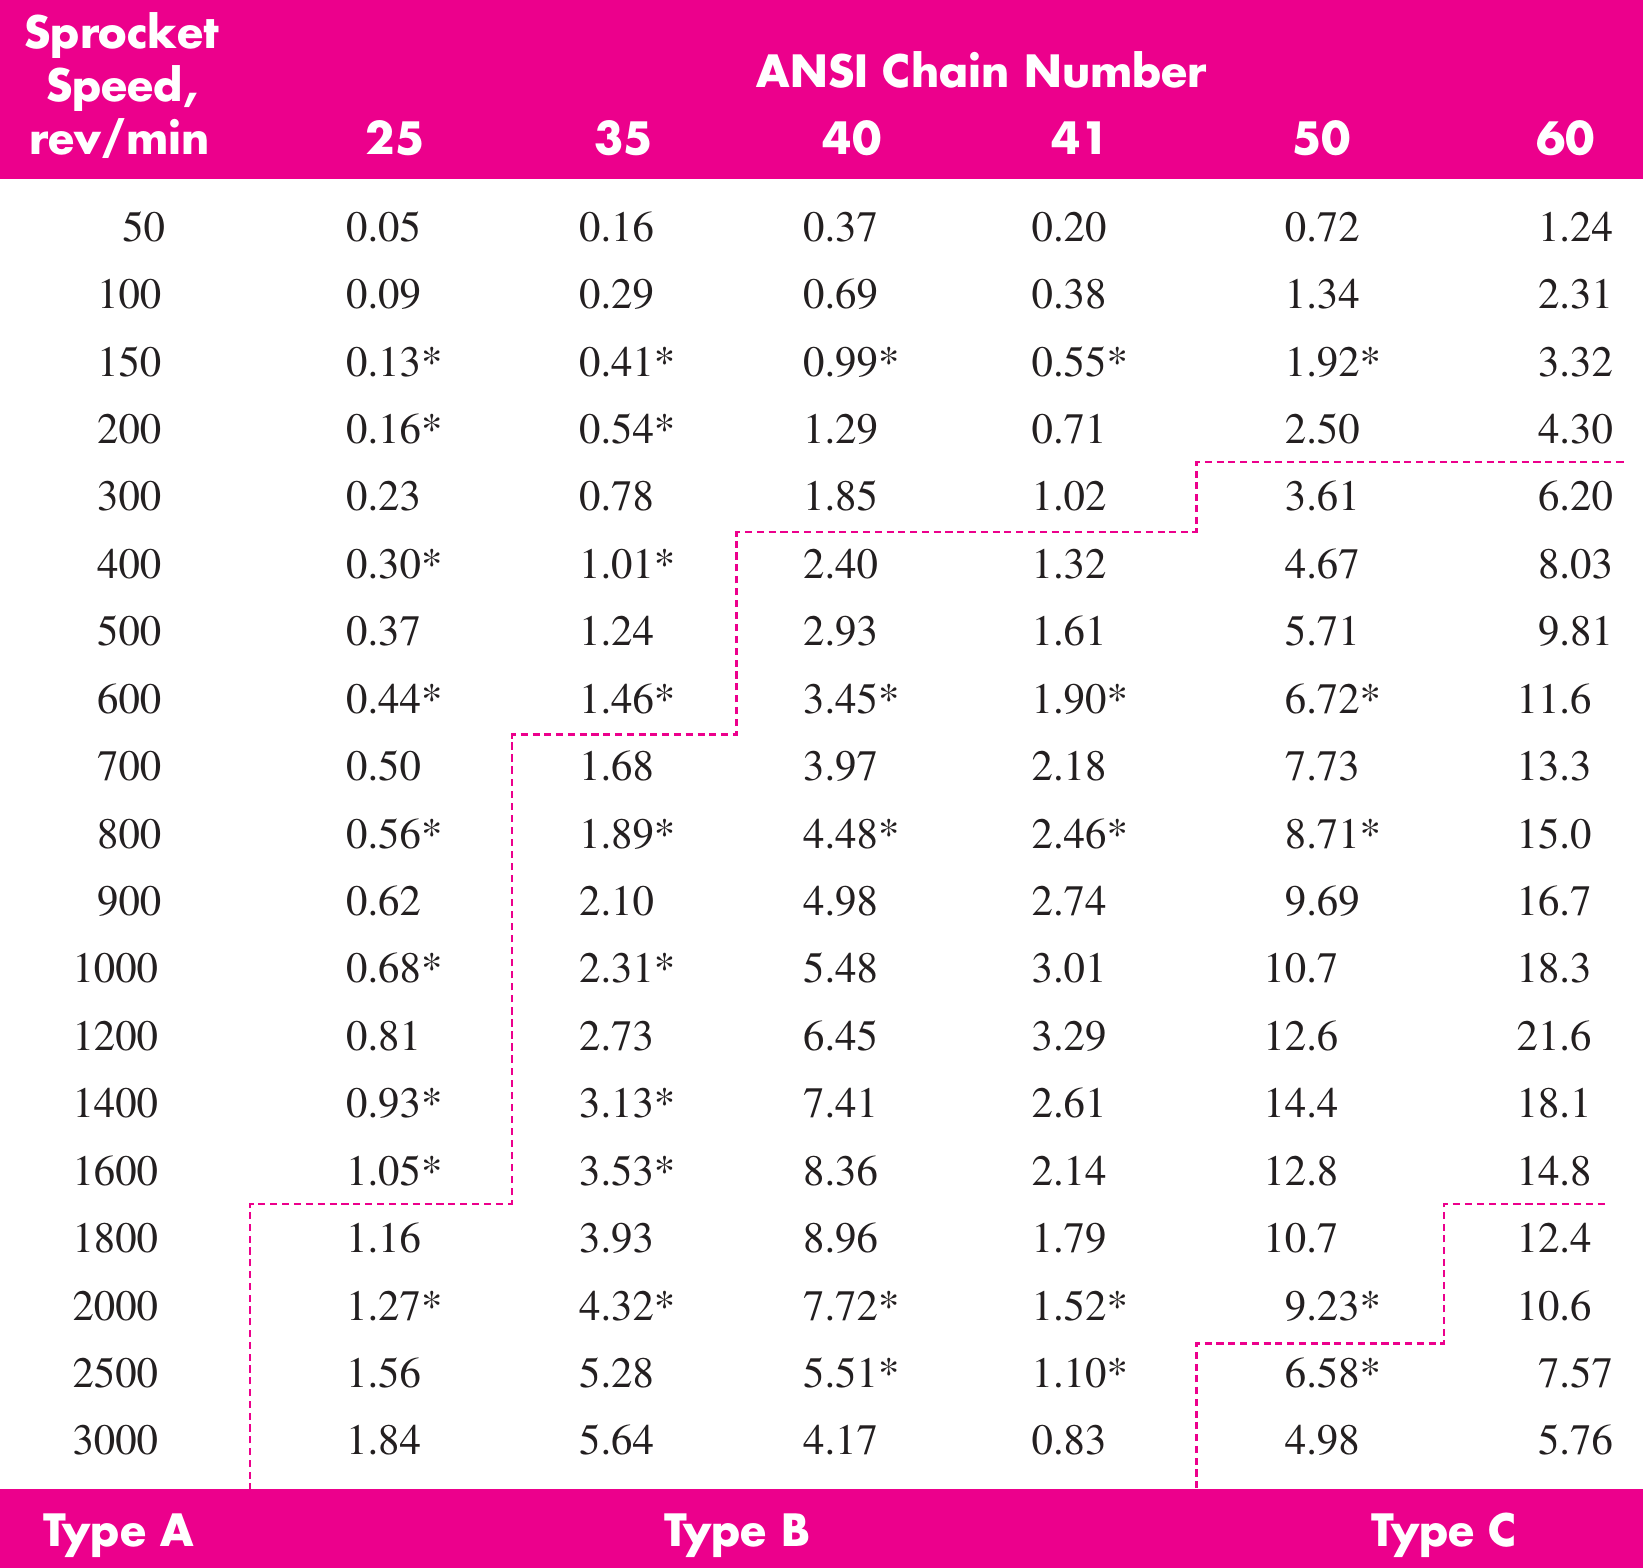
\includegraphics[width=0.8\textwidth]{./pictures/chain-rated-capacity.png}
\end{center}
\end{frame}

\begin{frame}[label={sec:orgb63fbc6}]{Roller Chain Rated Capacity in hp (2)}
\begin{center}
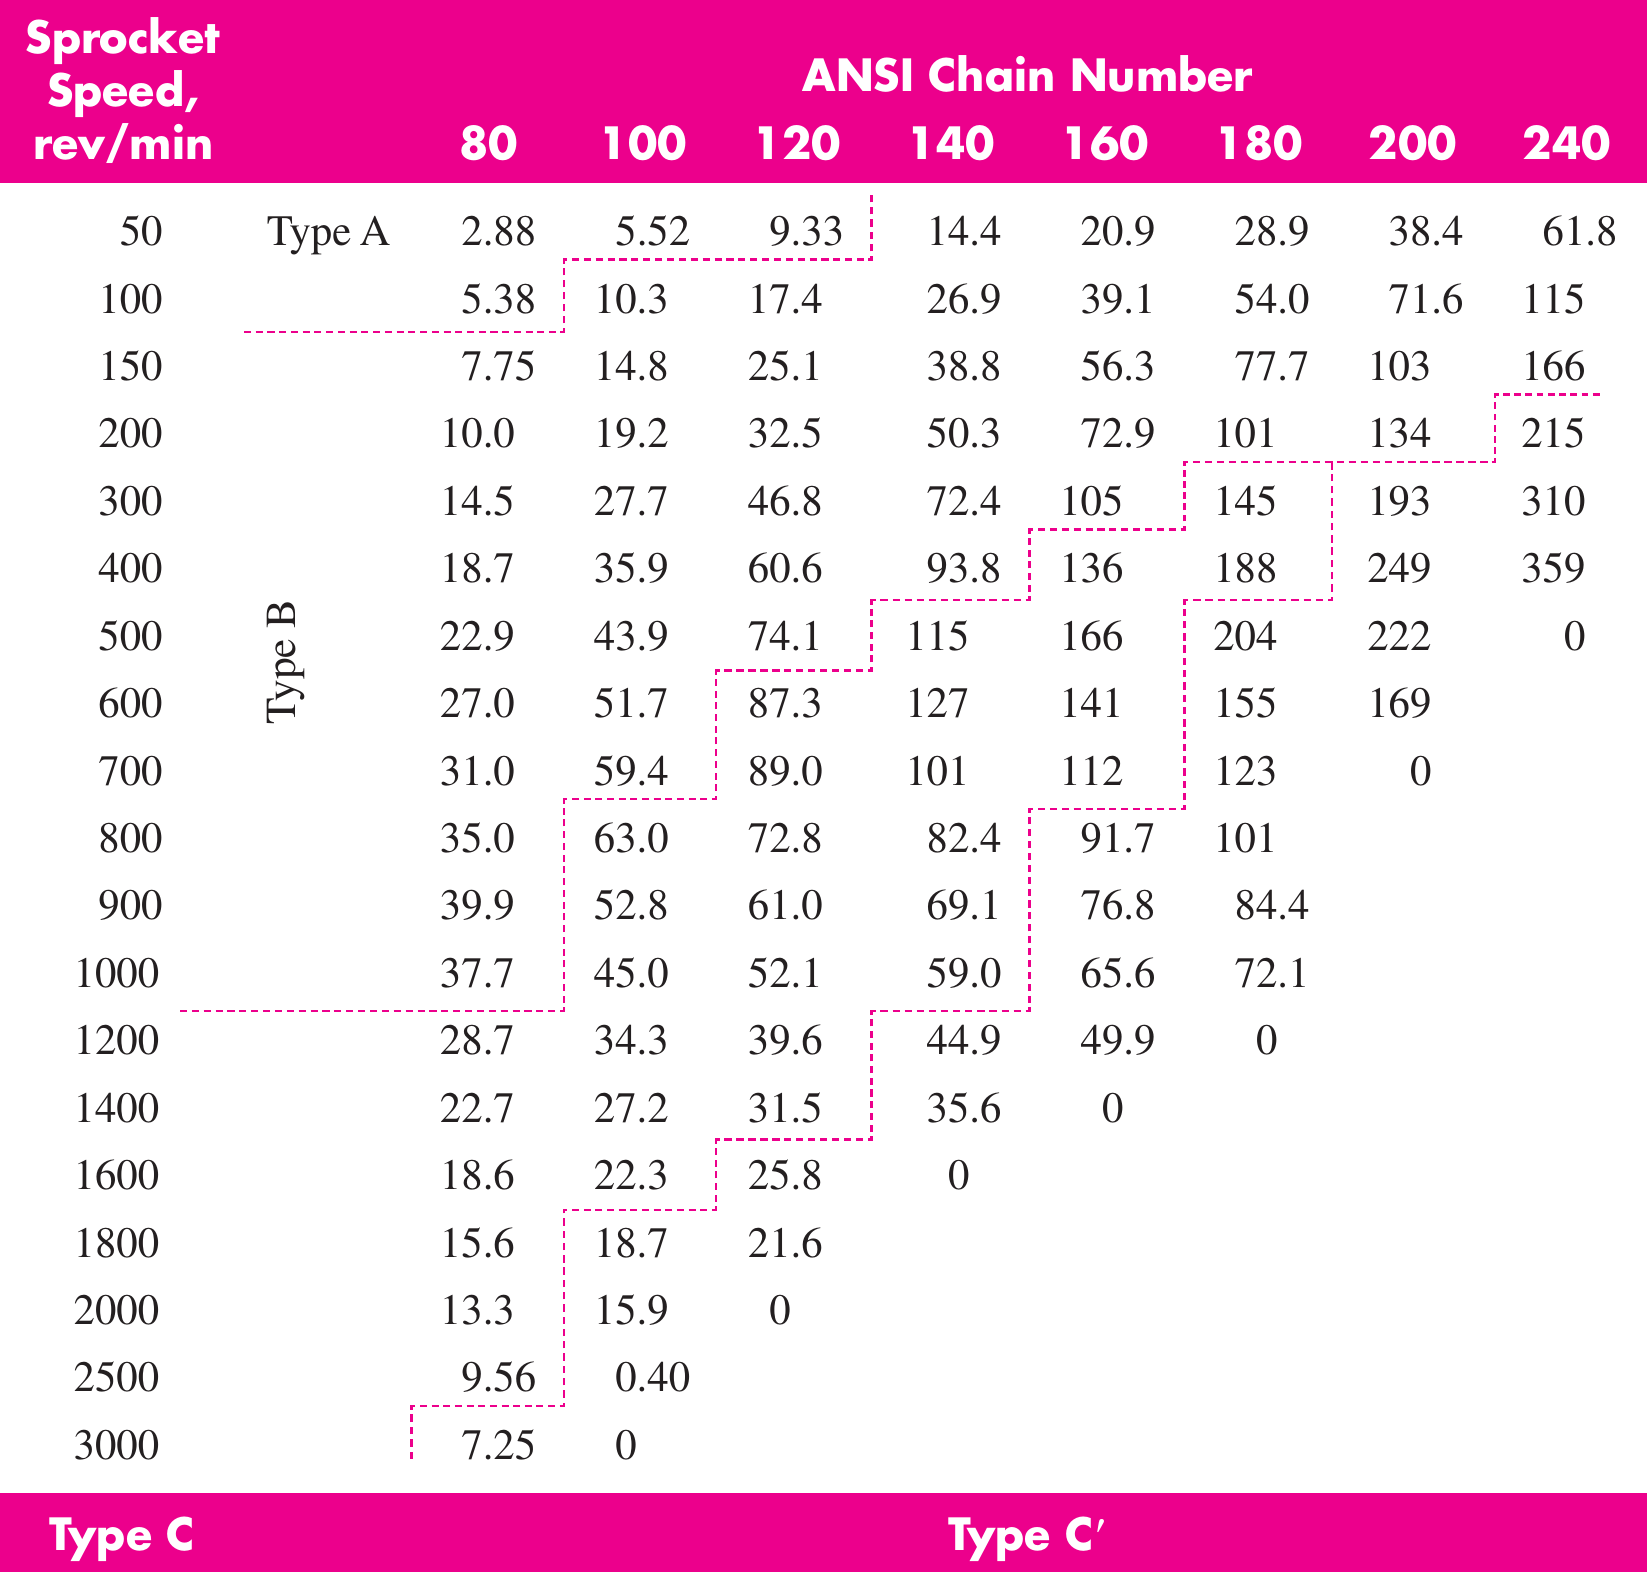
\includegraphics[width=0.8\textwidth]{./pictures/chain-rated-capacity2.png}
\end{center}
\end{frame}

\begin{frame}[label={sec:org8d3ca2f}]{Example}
Pick a roller chain for a motorcycle whose output engine is 15 hp at 1000 rpm. The driving sprocket has 20 teeth and the output has 39 teeth.
\end{frame}

\begin{frame}[label={sec:org753c2e6}]{Solution}
For 15 hp at 1000 rpm, try ANSI 60. p = 0.75 in

\begin{align*}
    H_1 &= 0.003(20)^{1.08}(1000)^{0.9}(0.75)^{3-0.07(0.75)} \\
        &= 21.8 \text{ kW} \\
    H_2 &= \frac{1000(17)(20)^{1.5}(0.75)^{0.8}}{1000^{1.5}} \\
        &= 38.2 \text{ kW}
\end{align*}

This means the chain can deliver the power with the safety factor of 21.8/15 = 1.45
\end{frame}
\end{document}